\documentclass[11pt,american,american]{article}
\usepackage[a4paper]{geometry}
\geometry{verbose,tmargin=2cm,bmargin=2cm,lmargin=2cm,rmargin=2cm,headheight=0.8cm,headsep=1cm,footskip=0.5cm}
\setcounter{secnumdepth}{3}
\usepackage{url}
\usepackage{amsmath}
\usepackage{amsthm}
\usepackage{amssymb}
\usepackage{graphicx}
\usepackage{setspace}
\usepackage{enumerate} %roman enumiration
\usepackage{threeparttable}
\usepackage{algorithmic}
\usepackage{algorithm}
\usepackage{subfigure}
\usepackage[width=.75\textwidth]{caption}
\usepackage{array}
\usepackage[utf8]{inputenc} % Required for inputting international characters
\usepackage[T1]{fontenc} % Output font encoding for international characters
\usepackage{mathpazo} % Palatino font
\usepackage{multirow}
\usepackage{chngcntr}

\counterwithin{figure}{section}
\counterwithin{table}{section}

\pagenumbering{arabic}

\makeatletter
%%%%%%%%%%%%%%%%%%%%%%%%%%%%%% Algorithms
% Define a \HEADER{Title} ... \ENDHEADER block
\newcommand{\HEADER}[1]{\ALC@it\underline{\textsc{#1}}\begin{ALC@g}}
	\newcommand{\ENDHEADER}{\end{ALC@g}}
\renewcommand*{\ALG@name}{Algoritmus}
\algsetup{indent=2em} 
\renewcommand{\algorithmiccomment}[1]{\hspace{2em}// #1} 
\makeatother

%% Use Times New Roman font for text and Belleek font for math
%% Please make sure that the 'esint' package is turned off in the
%% 'Math options' page.
\usepackage[varg]{txfonts}


%% Indent even the first paragraph in each section
\usepackage{indentfirst}

% completely avoid orphans (first lines of a new paragraph on the bottom of a page)
\clubpenalty=9500

% completely avoid widows (last lines of paragraph on a new page)
\widowpenalty=9500

% disable hyphenation of acronyms
\hyphenation{CDFA HARDI HiPPIES IKEM InterTrack MEGIDDO MIMD MPFA DICOM ASCLEPIOS MedInria}

%%---------------------------------------------------------------------

%% Print out all vectors in bold type instead of printing an arrow above them
%%\renewcommand{\vec}[1]{\boldsymbol{#1}}

% Replace standard \cite by the parenthetical variant \citep
%\renewcommand{\cite}{\citep}

\makeatother
%\pagestyle{empty} %turns off page numbering
\usepackage{babel}
\newcommand*\Laplace{\mathop{}\!\mathbin\bigtriangleup}
\newcommand*\midpoint[1]{\overline{#1}}

\begin{document}
\selectlanguage{american}
\def\documentdate{...}


\begin{titlepage} % Suppresses displaying the page number on the title page and the subsequent page counts as page 1
	\newcommand{\HRule}{\rule{\linewidth}{0.5mm}} % Defines a new command for horizontal lines, change thickness here
	\center % Centre everything on the page	
	
	\textsc{\LARGE FNSPE CTU}\\[1.5cm] % Main heading such as the name of your university/college
	\vfill
%	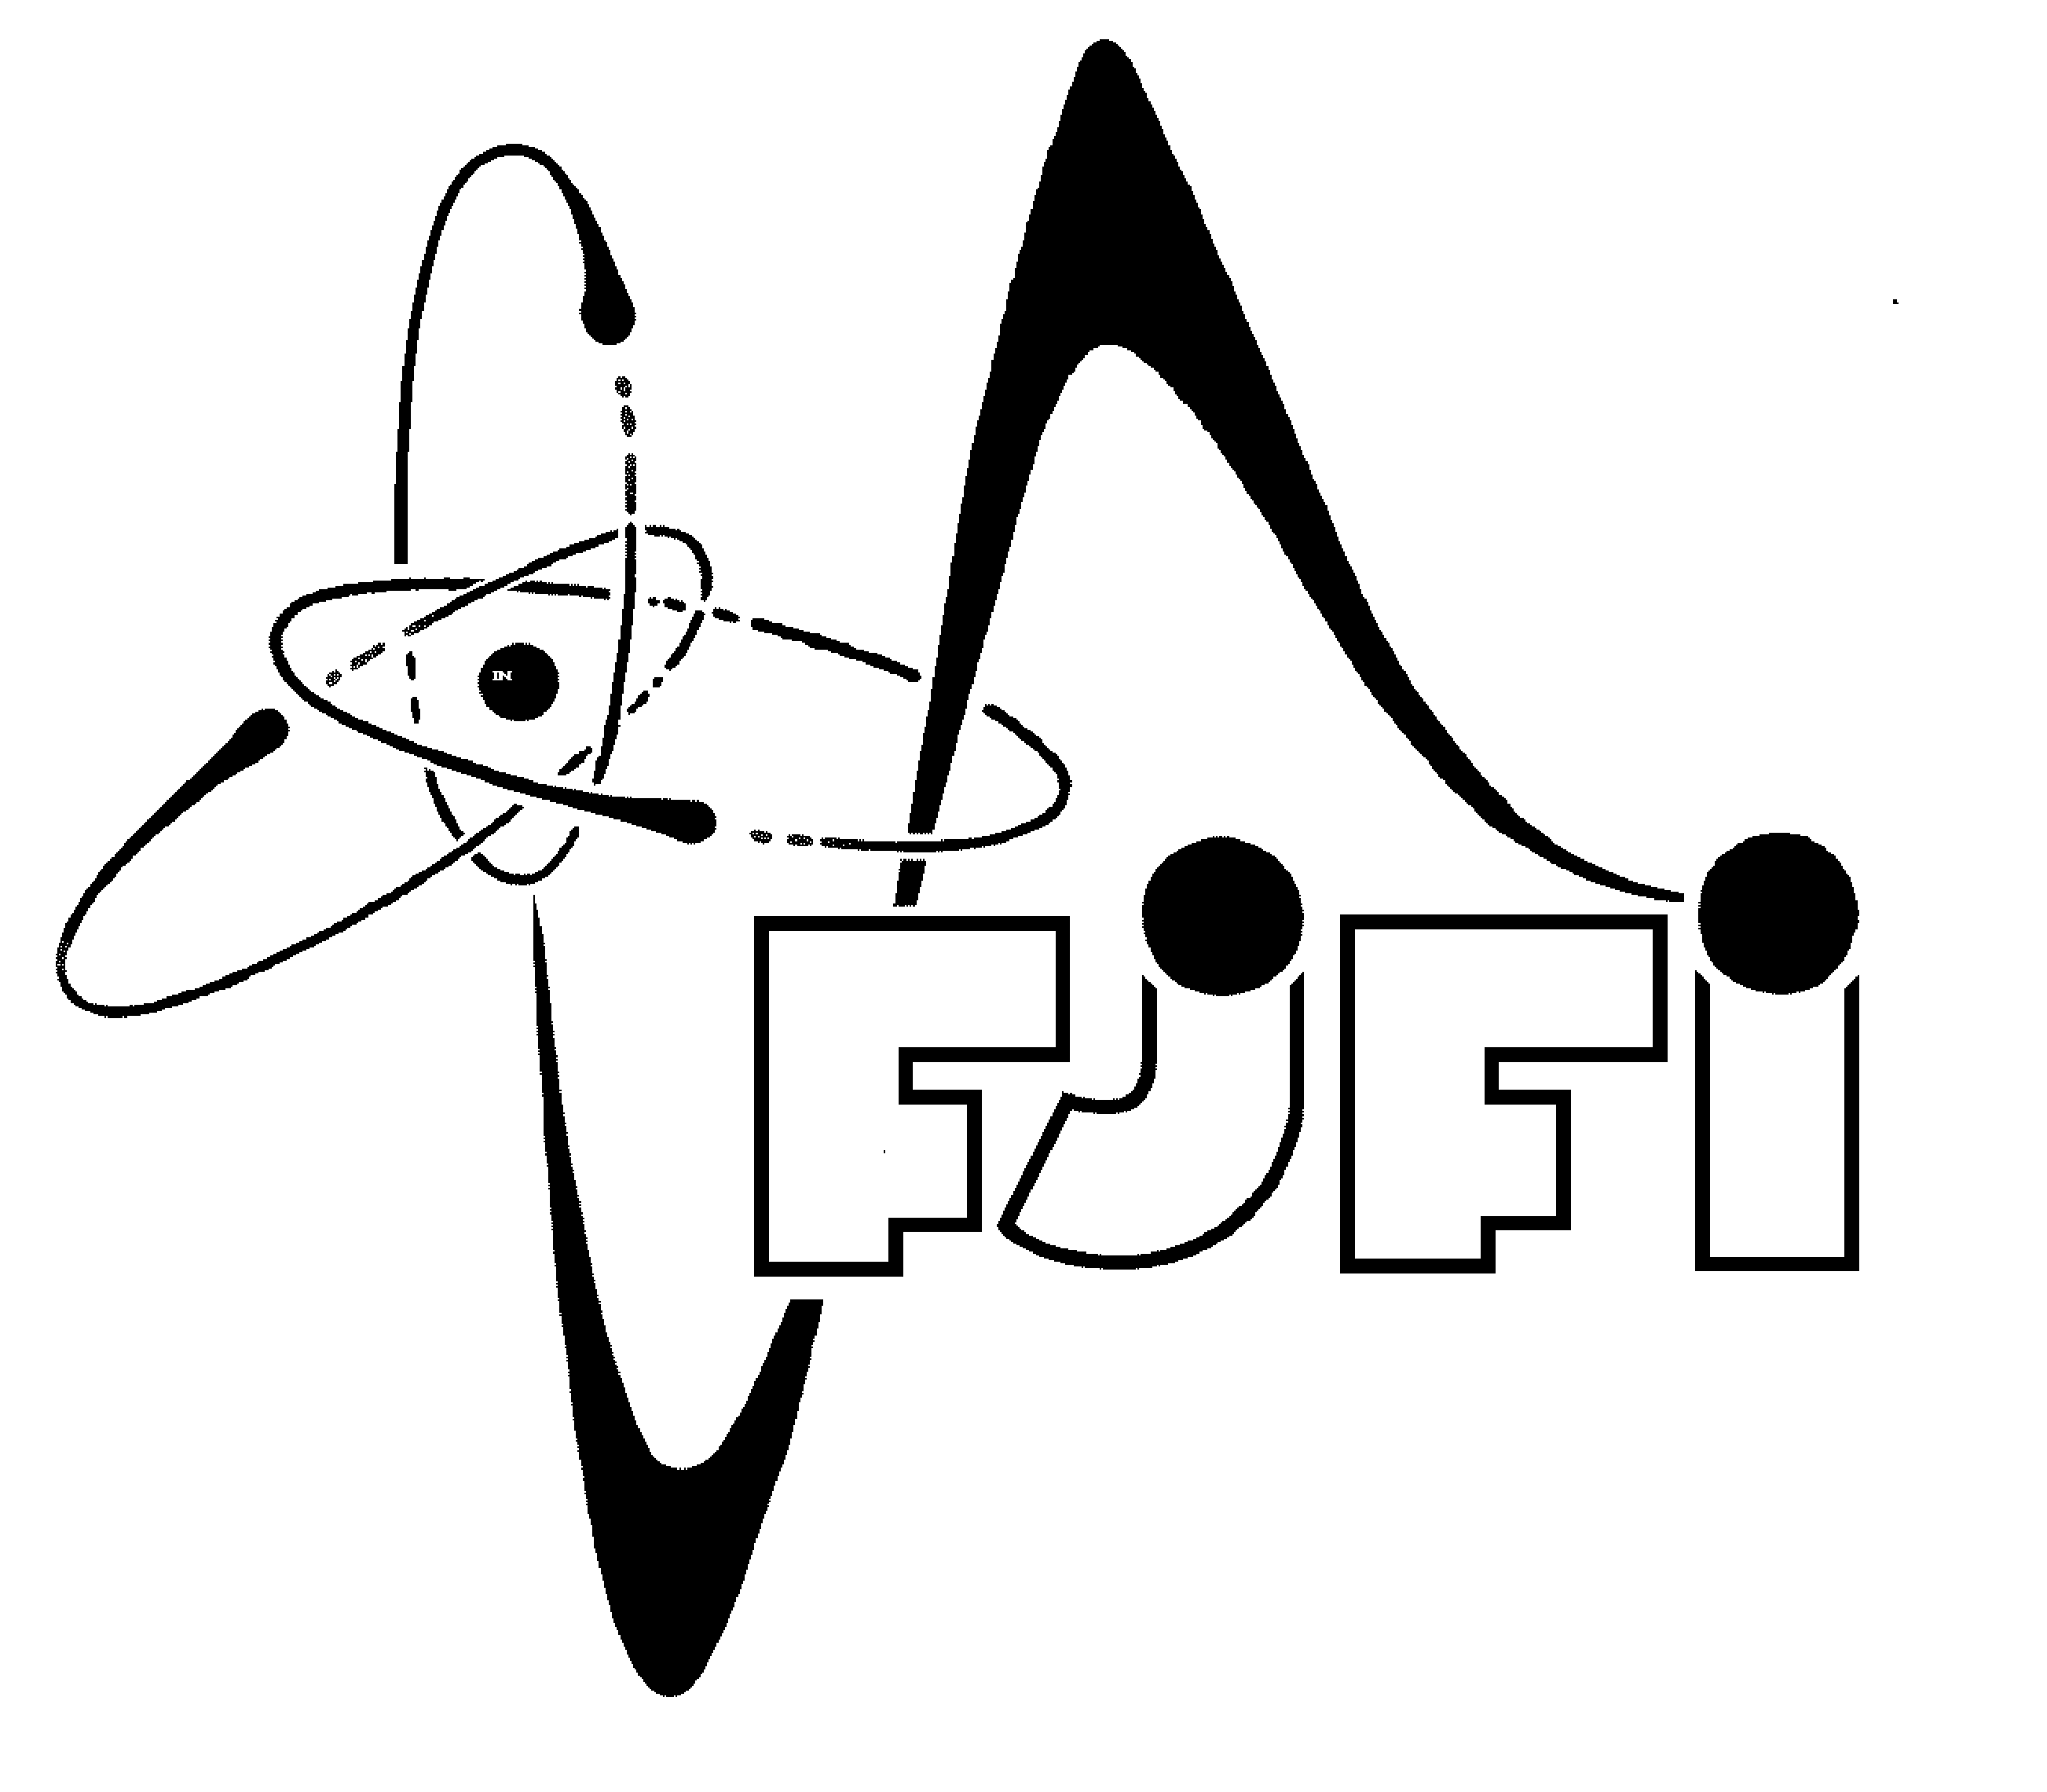
\includegraphics[width=0.2\textwidth]{Images/TITLE/fjfi}\\[1cm] % Include a department/university logo - this will require the graphicx package	
	
%	\noindent %
%	\begin{minipage}[c]{3cm}%
%		\noindent \begin{center}
%			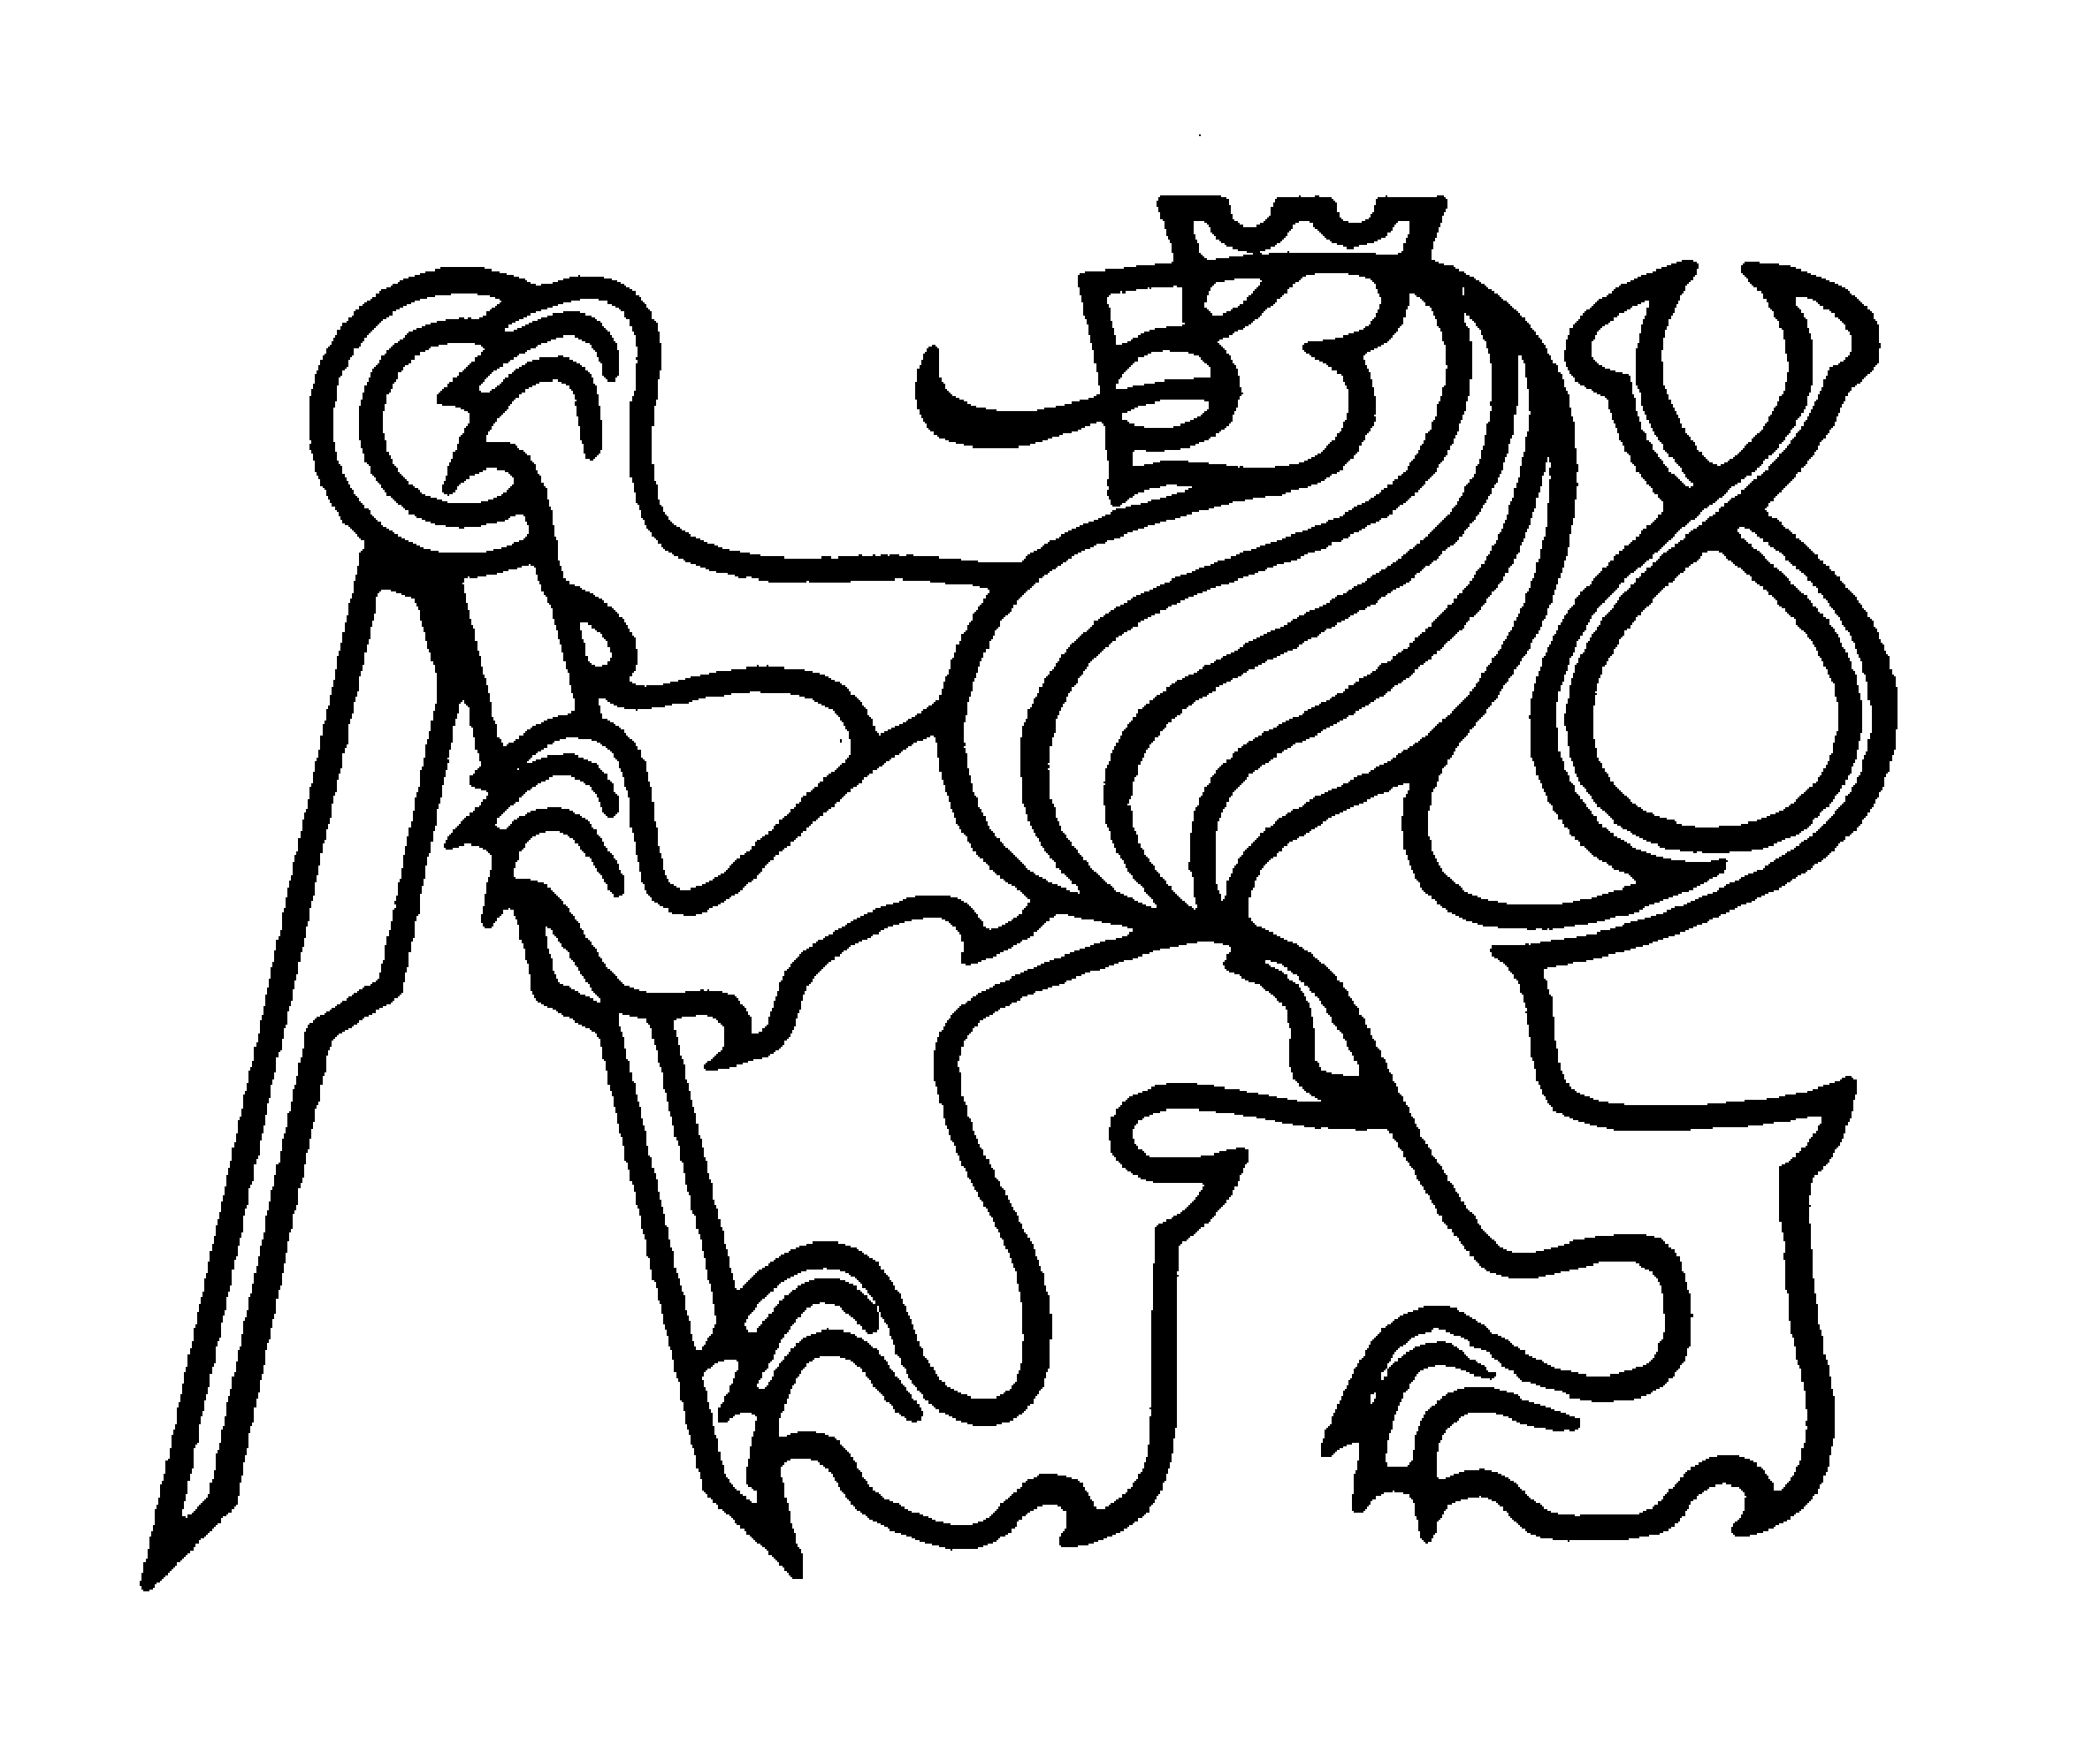
\includegraphics[width=3cm,height=3cm,keepaspectratio]{Images/TITLE/cvut}
%			\par\end{center}%
%	\end{minipage}%
%	\begin{minipage}[c]{0.6\linewidth}%
%		\begin{center}
%			\textsc{\large{}České vysoké učení technické v Praze}{\large{}}\\
%			{\large{}Fakulta jaderná a fyzikálně inženýrská}
%			\par\end{center}%
%	\end{minipage}%
%	\begin{minipage}[c]{3cm}%
%		\noindent \begin{center}
%		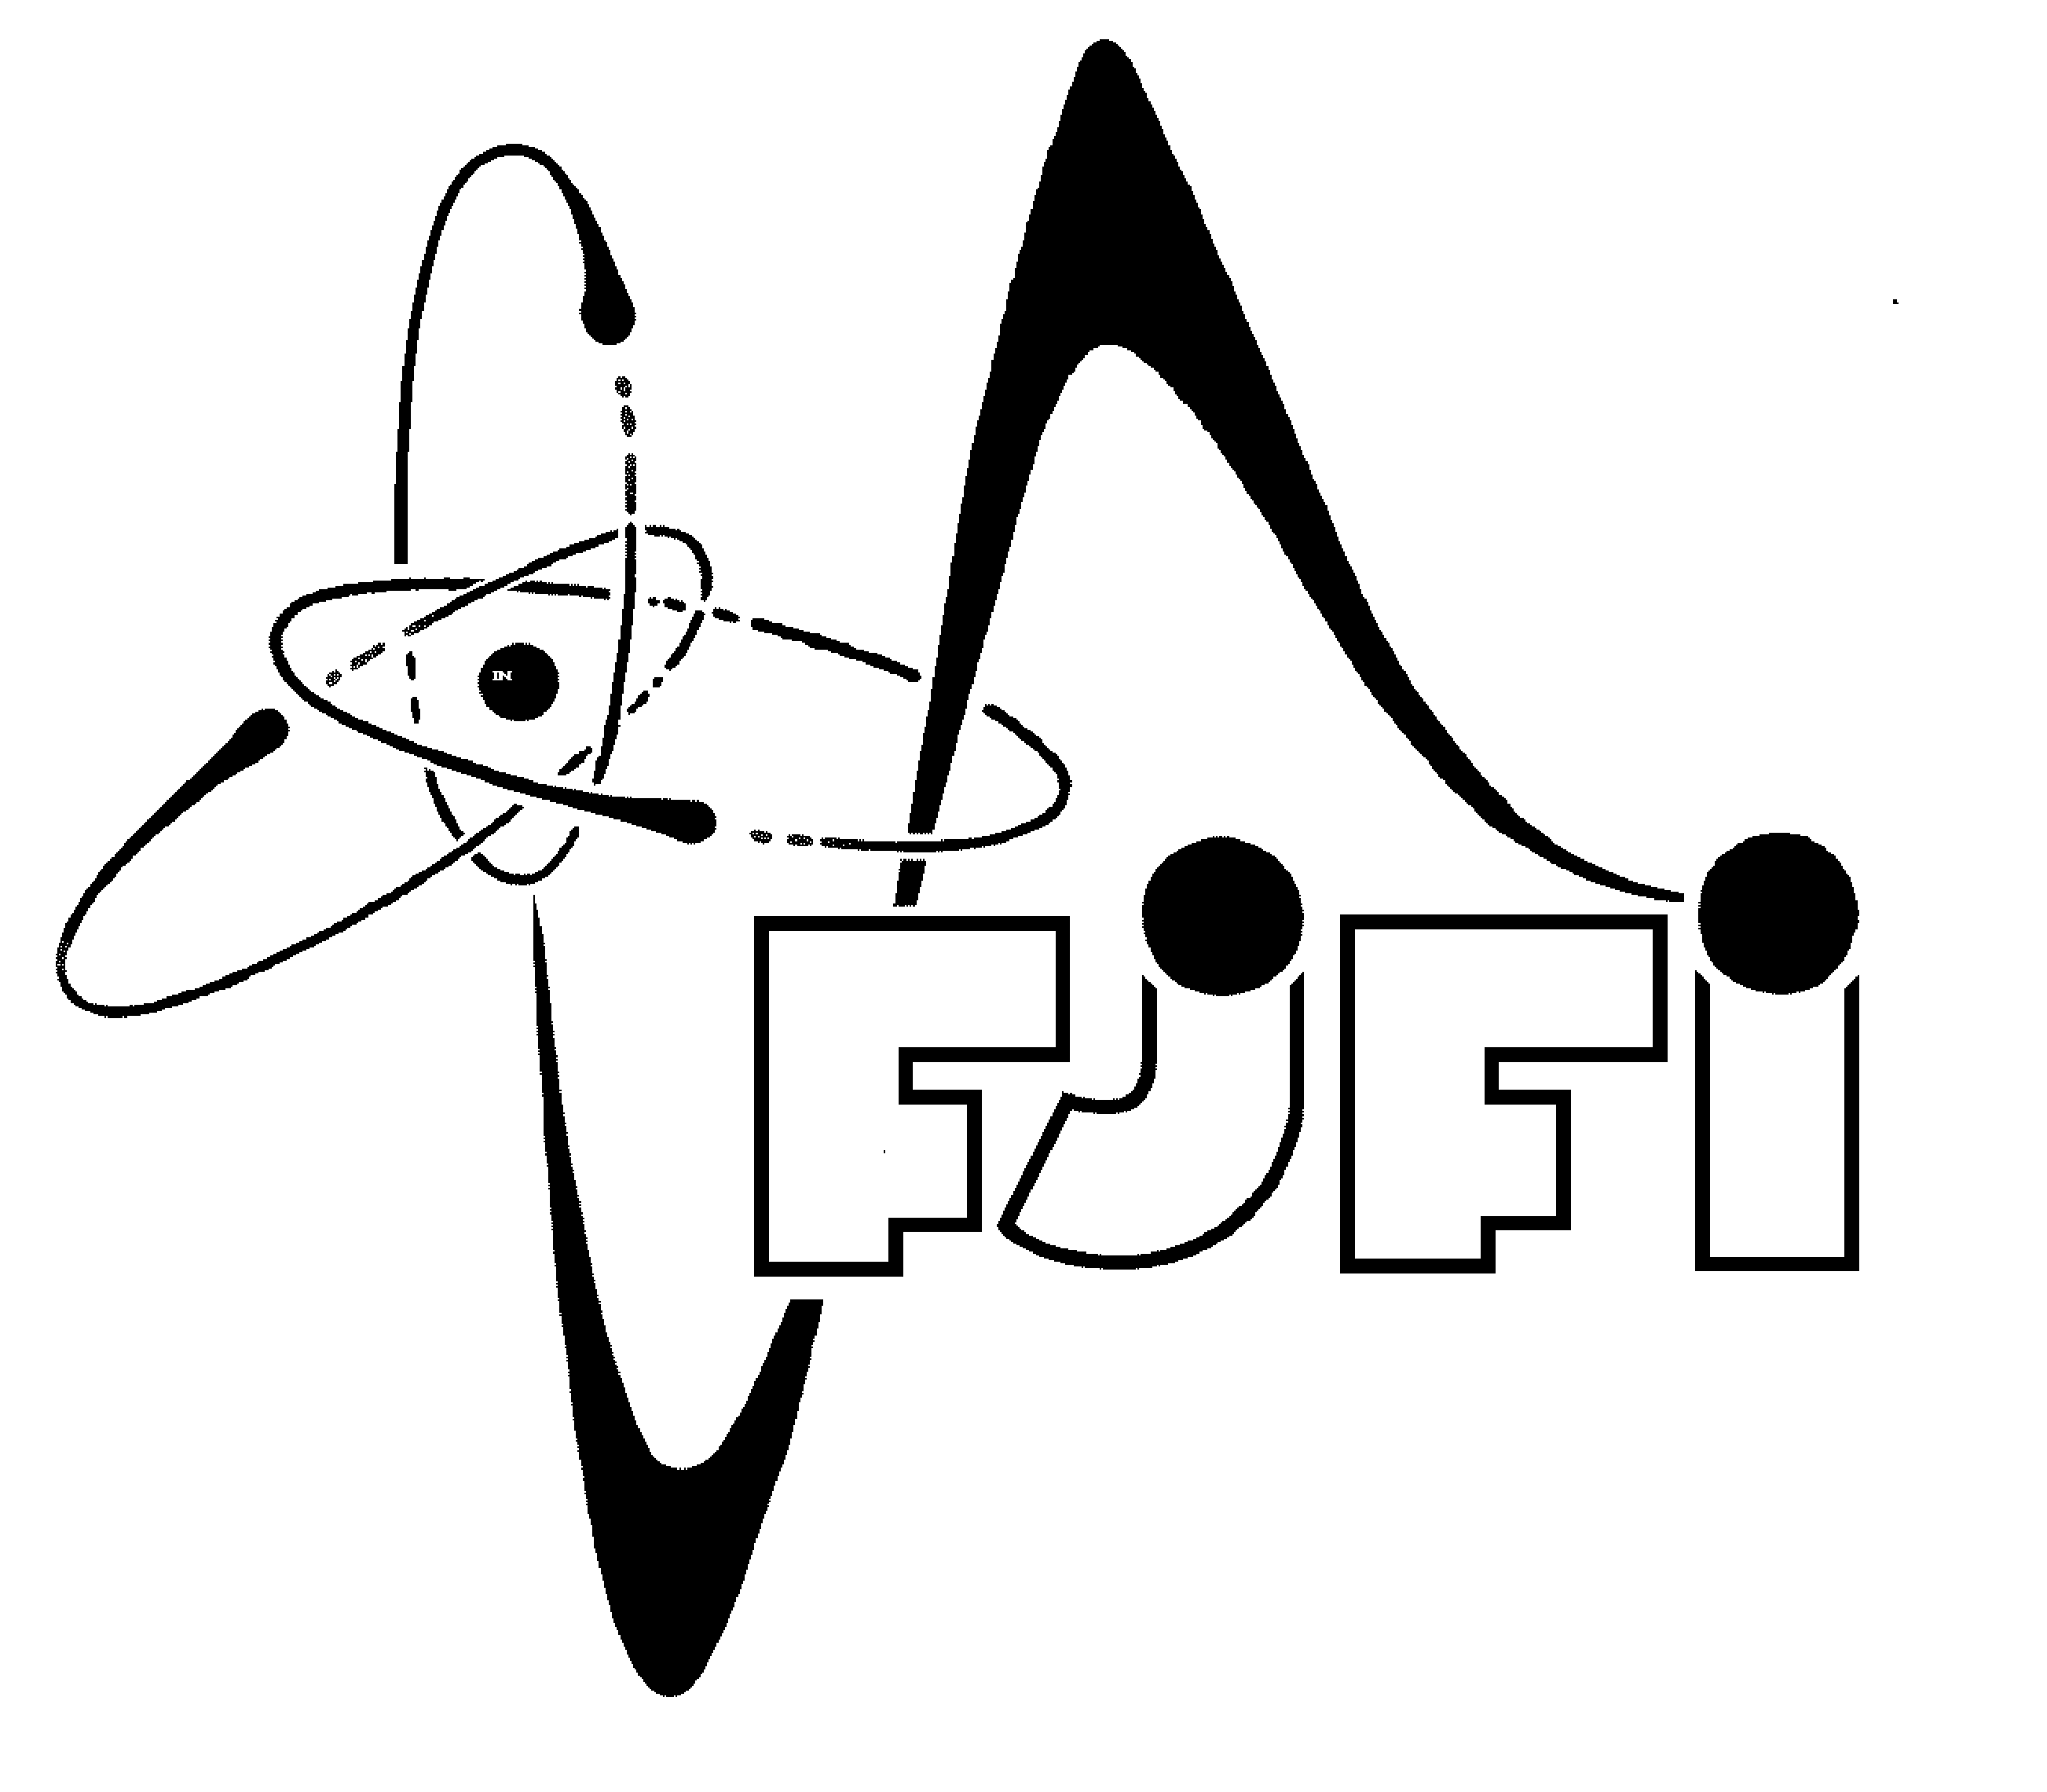
\includegraphics[width=3cm,height=3cm,keepaspectratio]{Images/TITLE/fjfi}
%		\par\end{center}%
%	\end{minipage}
%	\vspace{3cm}
	
	\textsc{\Large ASM}\\[0.5cm] % Major heading such as course name
	\textsc{\large Dataset n.6}\\[0.5cm] % Minor heading such as course title
	\HRule\\[0.4cm]
	{\huge\bfseries Fitting Percentage of Body Fat to Simple Body Measurements}\\[0.4cm] % Title of your document
	\HRule\\[1.5cm]
	{\large\textit{Author:}}\\
	Vladislav \textsc{Belov}\\
	\vfill\vfill\vfill\vfill\vfill\vfill\vfill % Position the date 3/4 down the remaining page
	{\large\today} % Date, change the \today to a set date if you want to be precise
	
	%------------------------------------------------
	%	Logo
	%------------------------------------------------
	
%	\vfill\vfill
%	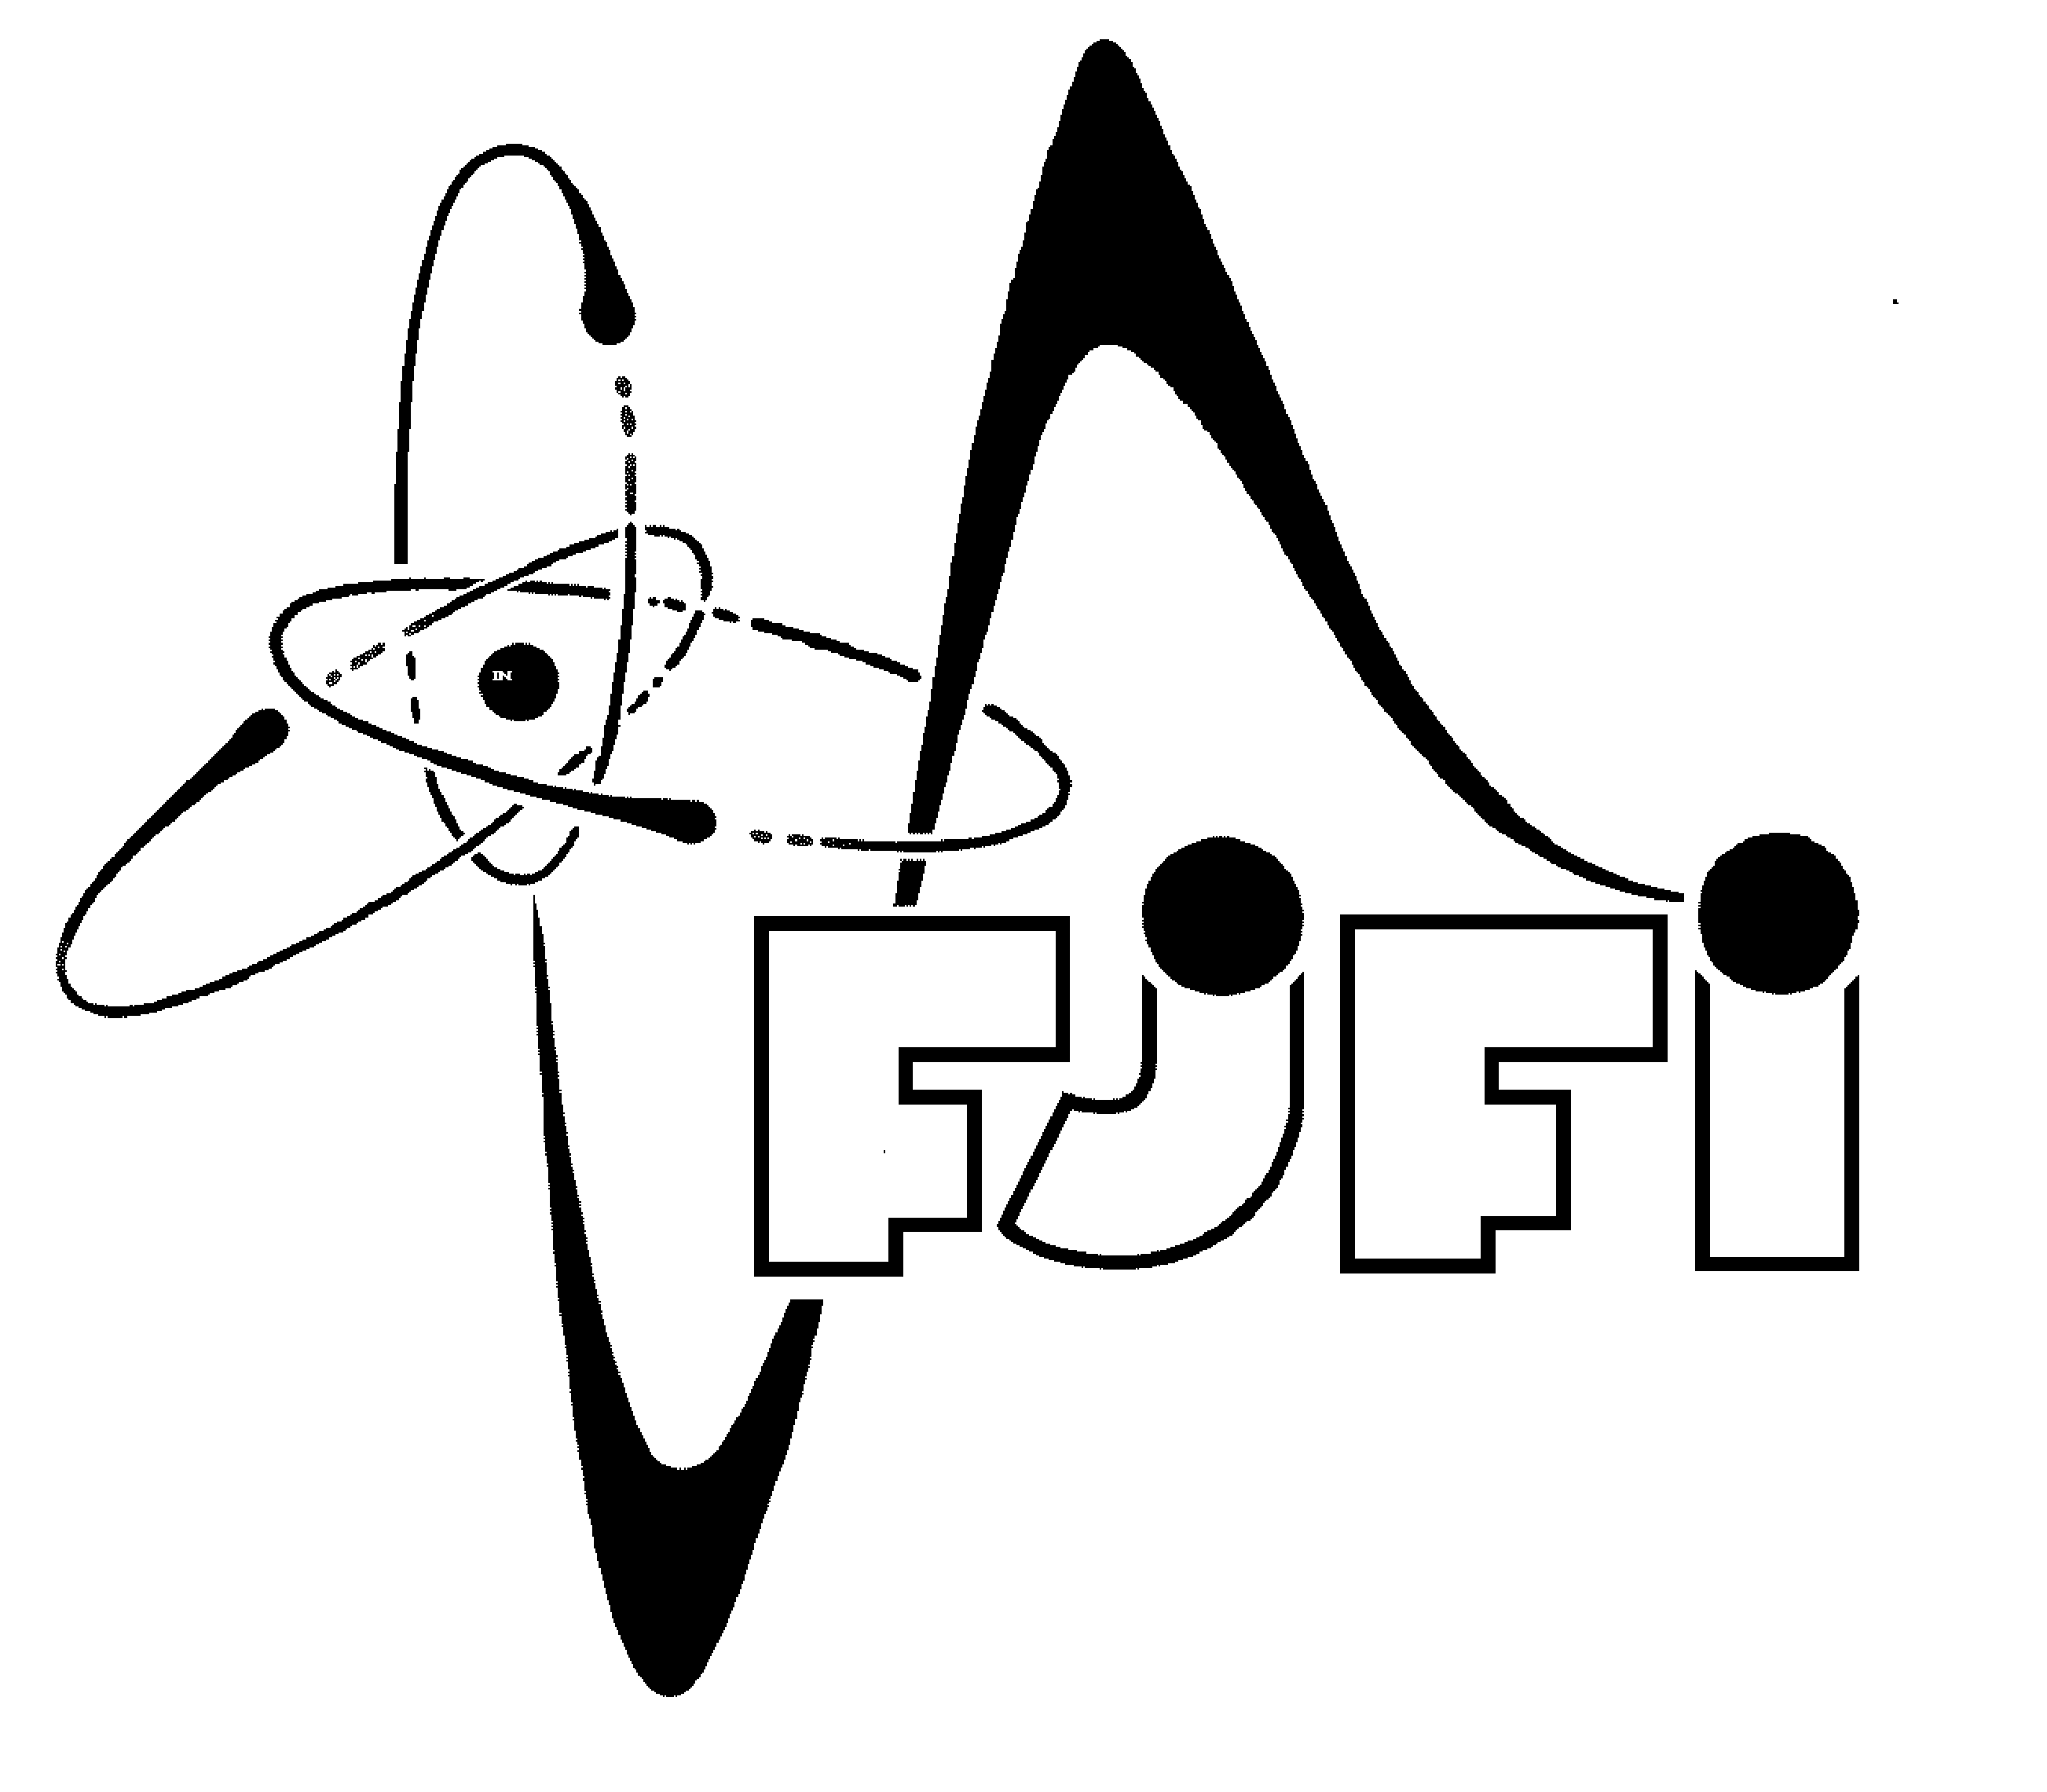
\includegraphics[width=0.2\textwidth]{Images/TITLE/fjfi}\\[1cm] % Include a department/university logo - this will require the graphicx package
%	
	%----------------------------------------------------------------------------------------
	
	\vfill % Push the date up 1/4 of the remaining page
	
\end{titlepage}

%\tableofcontents
%\newpage{}

\section{Outline}\label{sec:outline}

In this paper we will perform an analysis of the dataset which contains simple measurements of $252$ men. Circumferences of body parts, age, weight and fat percentage are a part of the dataset. After providing descriptive statistics in section \ref{sec:desc} and performing a more detailed examination of some selected variables in section \ref{sec:analysis}, we will attempt to fit percentage of body fat to some of the body measurements in section \ref{sec:regression}. Body fat percentage can be measured using either Siri's equation or Brozek's equation:

\begin{equation*}
	\begin{split}
		\text{Siri: } \, &\frac{457}{\text{Body Density}} - 414.2,	\\ \\
		\text{Brozek: } \, &\frac{495}{\text{Body Density}} - 450.
	\end{split}
\end{equation*}

\section{Descriptive Statistics}\label{sec:desc}

\subsection{Numerical Analysis of Selected Variables}

In this section a general numerical overview of the dataset population is be provided. Basic information about population's weight and height is available in Tab.~\ref{tab:desc1}. Age is also considered a continuous instance, nevertheless, for illustrative purposes we have categorized it, and results can be seen in Tab.~\ref{tab:desc2}.\footnote{Inches were converted to centimeters, pounds to kilograms.} 

\medskip

\begin{table}[ht!]
	\centering
	\begin{tabular}{|c||c|c|c|c|c|c|}
		\hline 
		Variable &  Min. Value &  1st Quantile &  Median &  Mean Value &  3rd Quantile & Max. Value   \\ 
		\hline \hline 
		Total Weight, [kg] & 53.75 & 72.12 & 80.06 & 81.16 & 89.36 & 164.72   \\ 
		\hline 
		Fat-Free Weight, [kg] & 48.04 & 59.58 & 64.21 & 65.19 & 69.8 & 109.09   \\ 
		\hline 
		Height, [cm] & 74.93 & 173.35 & 177.8 & 178.18 & 183.51 & 197.49   \\ 
		\hline 
	\end{tabular} 
	\caption{Numerical descriptive statistics for weight and height of the population.}	
	\label{tab:desc1}
\end{table}

\begin{table}[ht!]
	\centering
	\begin{tabular}{|c||c|c|}
		\hline 
		Age & Count &  \%   \\ 
		\hline \hline 
		22-34 & 53 & 21.03   \\
		\hline
		35-49 & 116 & 46.03  \\
		\hline  
		50-64 & 62 &  24.6  \\
		\hline 
		65-81 & 21 &  8.34  \\
		\hline 
	
	\end{tabular} 
	\caption{Contingency table for age.}
	\label{tab:desc2}	
\end{table}
 
\subsection{Graphical Analysis of Selected Variables}

\subsection{Fat Percentage Analysis}

As body fat percentage is heavily dependent of body density, this section is opened by the histogram of it, see Fig.~\ref{fig:body_density_histogram}. Observing this diagram, we can speculate, that men with higher body weight have bodies with less density. Another noteworthy observation is that the histogram resembles normal distribution (Fig.~\ref{fig:density_fitdist}). However, more detailed analysis of this fact is provided in section \ref{sec:analysis}.

\medskip

In Fig.~\ref{fig:fat_percentage_boxplot} one can see the comparative diagram of fat percentage given by both Siri's and Brozek's equations. Similarities between them start to become noticeable. Moreover, looking at comparison of empirical cumulative distribution functions (see Fig.~\ref{fig:cdf_brozek_siri}), we can speculate, that they have similar distributions, besides, those distributions are normal, the fit is available in Fig.~\ref{fig:siri_fitdist}-\ref{fig:brozek_fitdist}. Relevant tests are carried out in section \ref{sec:analysis}.

\newpage

\vspace*{\fill}
\begin{figure}[H]
	\centering
	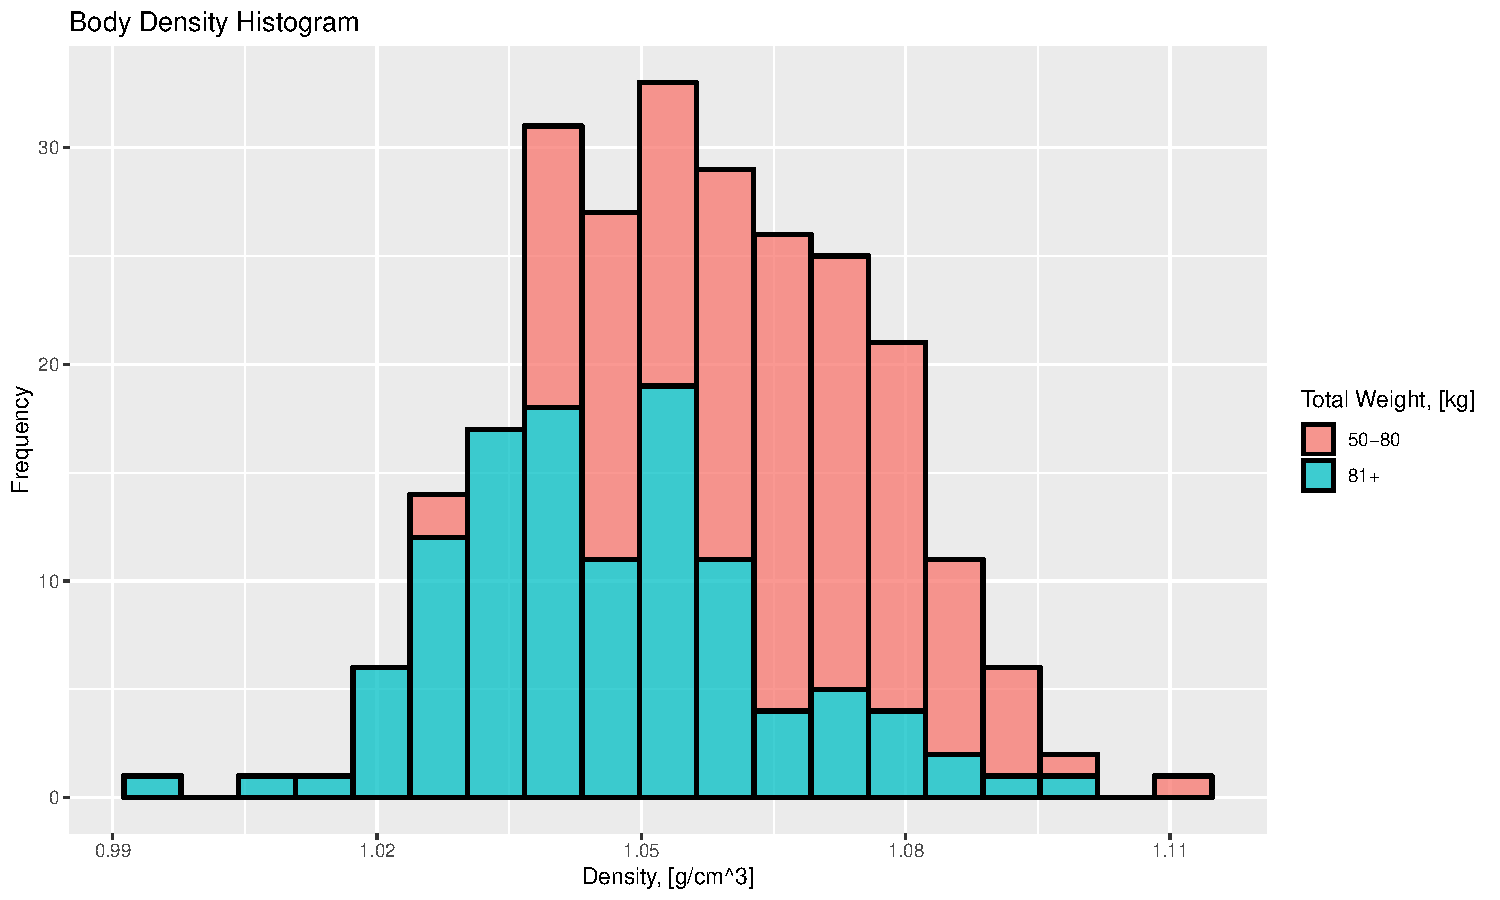
\includegraphics[width=0.75\linewidth]{Images/FIGURES/body_density_histogram}
	\caption{Body density histogram with categorized total weight for illustrative purposes.}
	\label{fig:body_density_histogram}
\end{figure}

\begin{figure}[H]
	\centering
	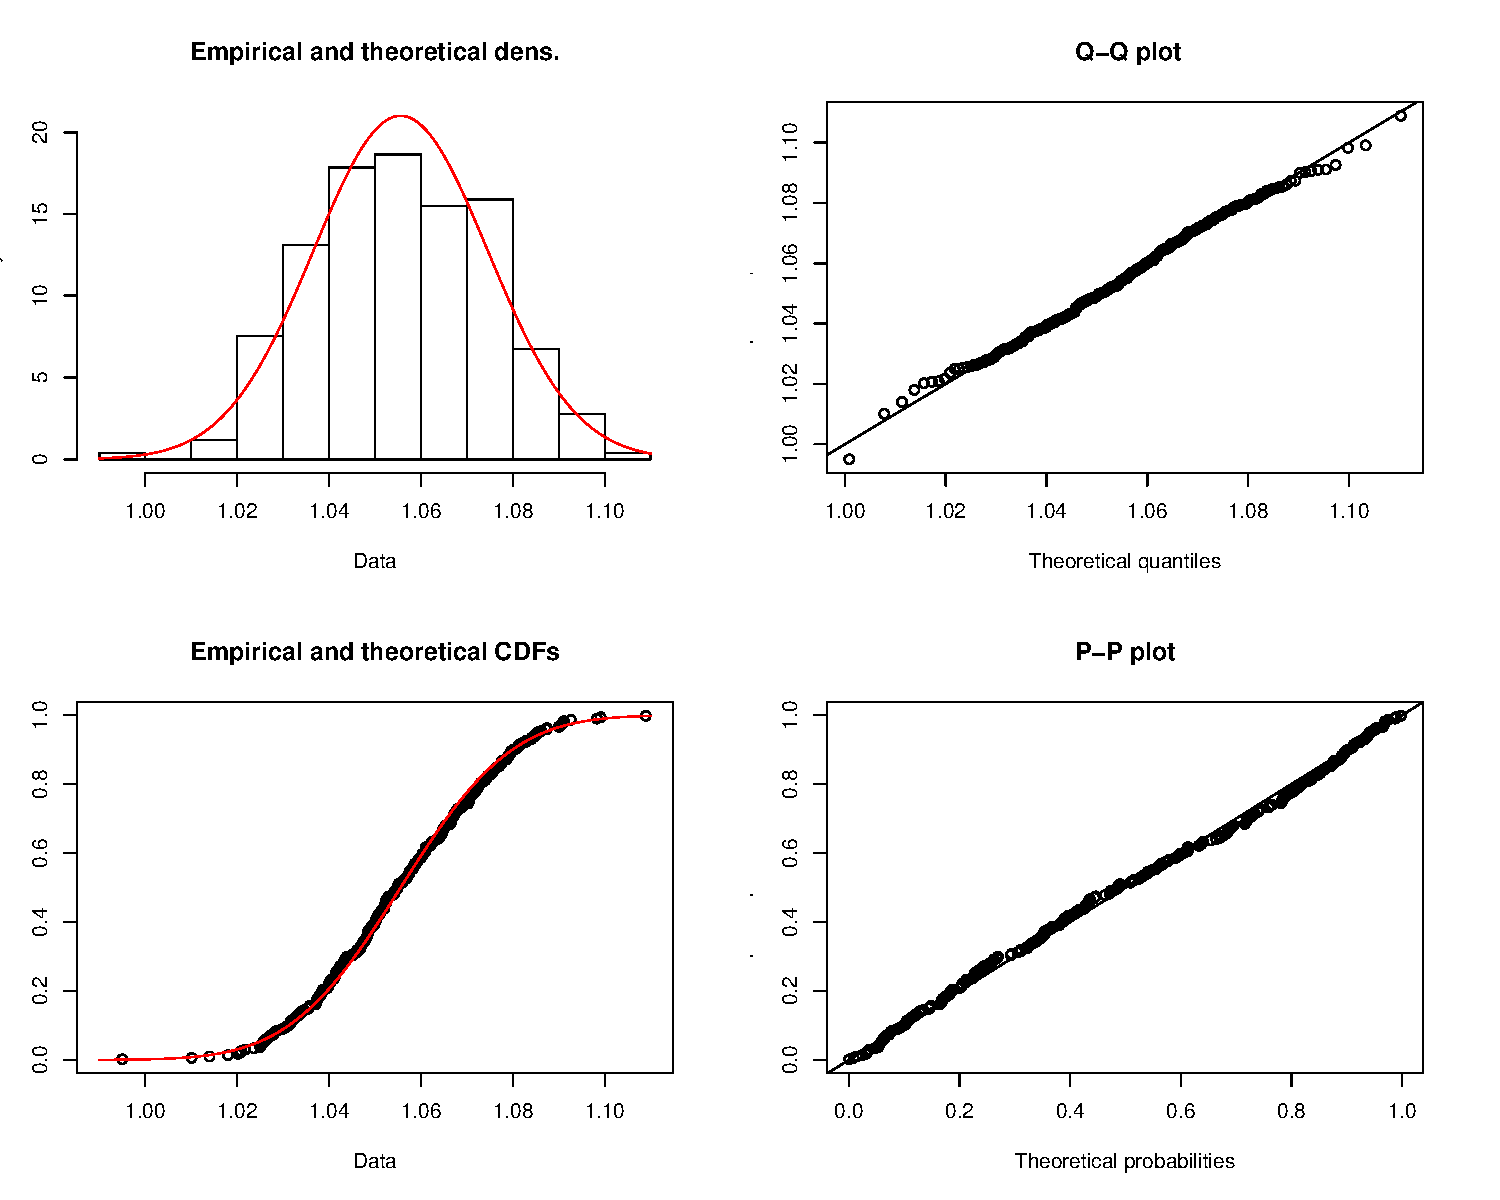
\includegraphics[width=0.8\linewidth]{Images/FIGURES/density_fitdist}
	\caption{Normal distribution fit to the body density.}
	\label{fig:density_fitdist}
\end{figure}
\vspace*{\fill}

\newpage

\begin{figure}[H]
	\centering
	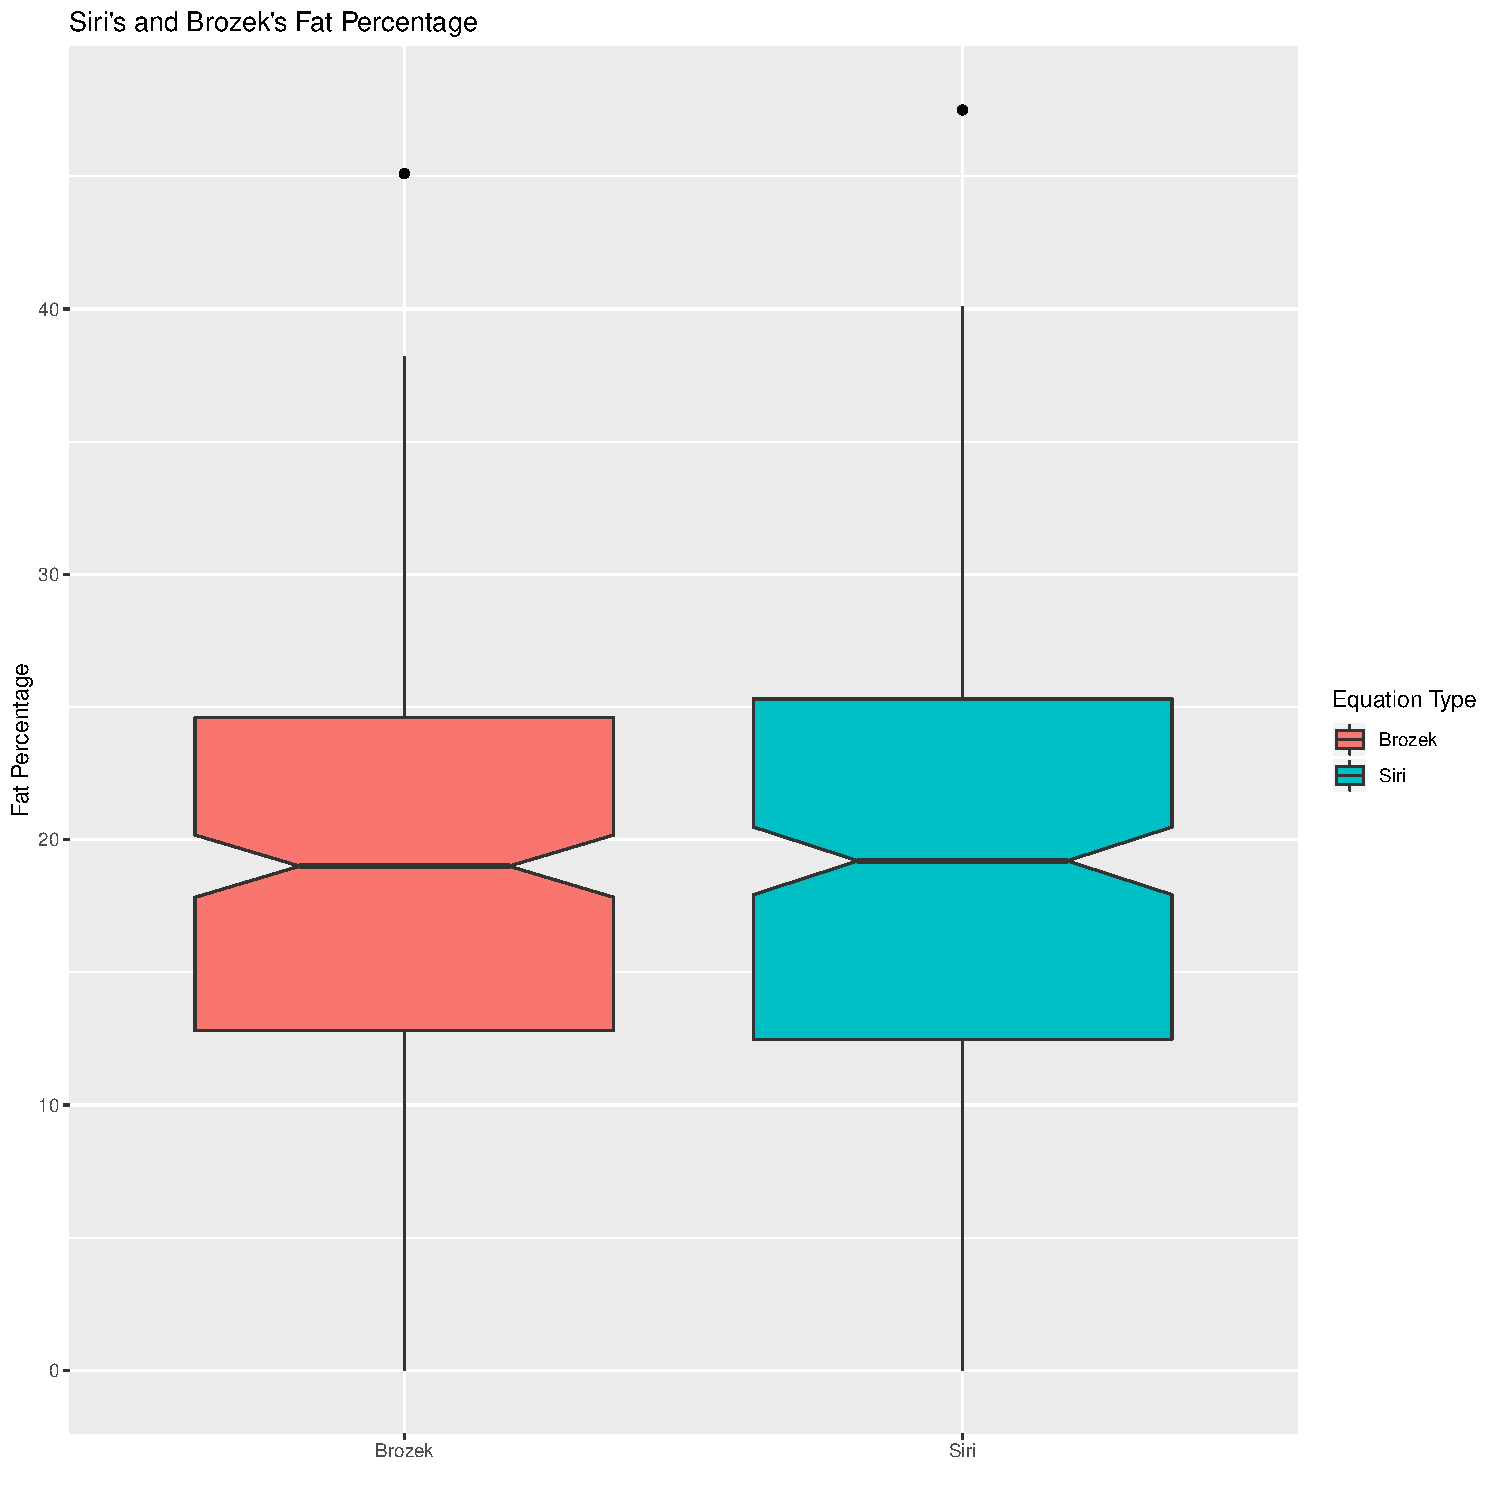
\includegraphics[width=0.7\linewidth]{Images/FIGURES/fat_percentage_boxplot}
	\caption{Comparative box plot of fat percentage given by Siri's and Brozek's equations.}
	\label{fig:fat_percentage_boxplot}
\end{figure}

\begin{figure}[H]
	\centering
	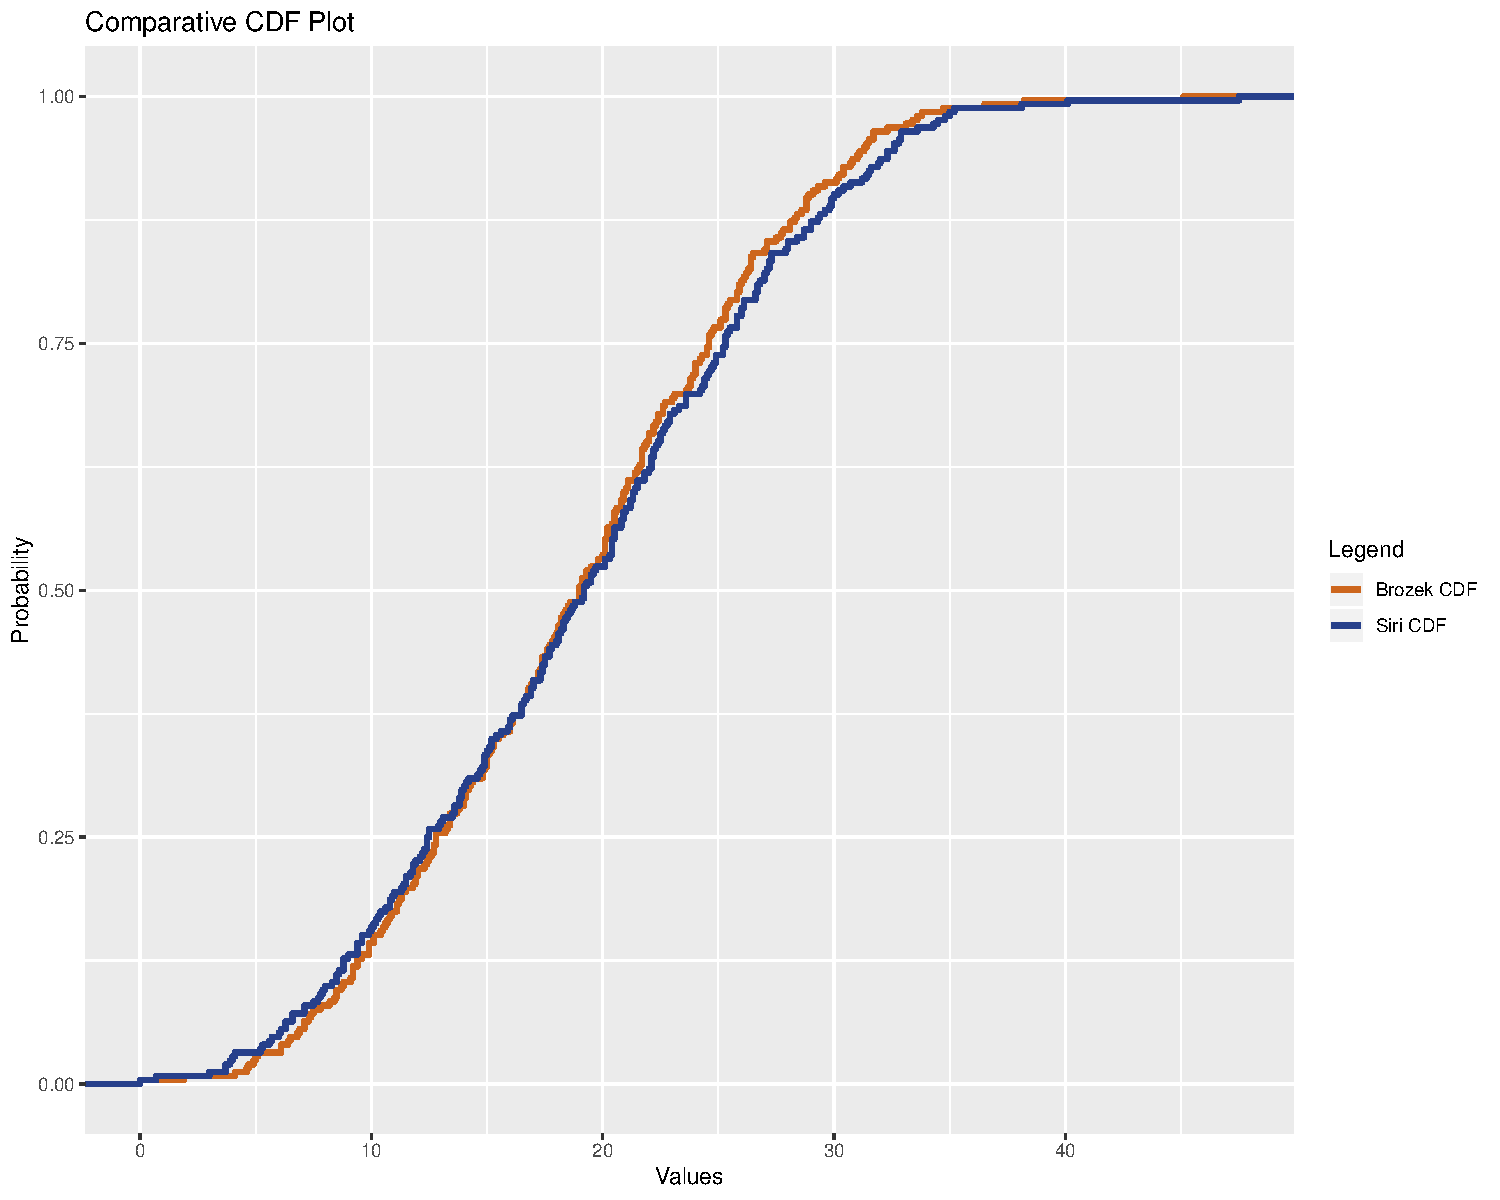
\includegraphics[width=0.75\linewidth]{Images/FIGURES/cdf_brozek_siri}
	\caption{Comparative plot of ECDFs for fat percentage given by Siri's and Brozek's equations.}
	\label{fig:cdf_brozek_siri}
\end{figure}

\newpage

\vspace*{\fill}
\begin{figure}[H]
	\centering
	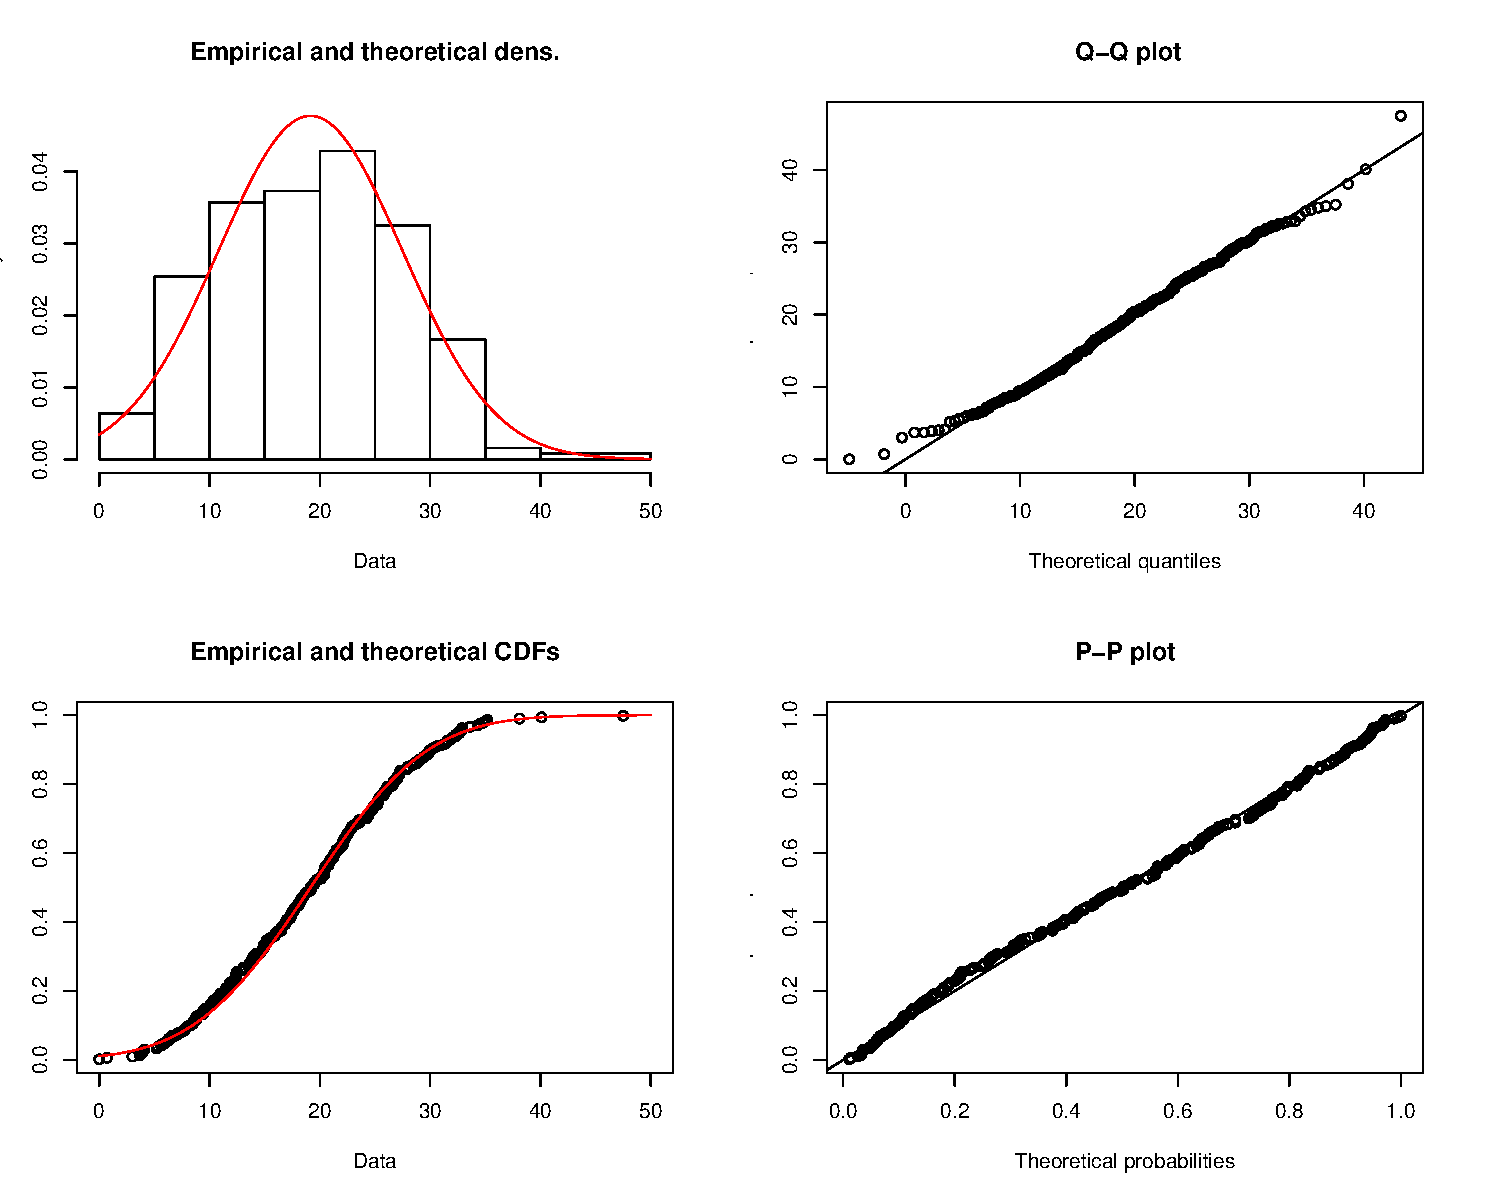
\includegraphics[width=0.8\linewidth]{Images/FIGURES/siri_fitdist}
	\caption{Normal distribution fit to fat percentage given by Siri's equation.}
	\label{fig:siri_fitdist}
\end{figure}

\begin{figure}[H]
	\centering
	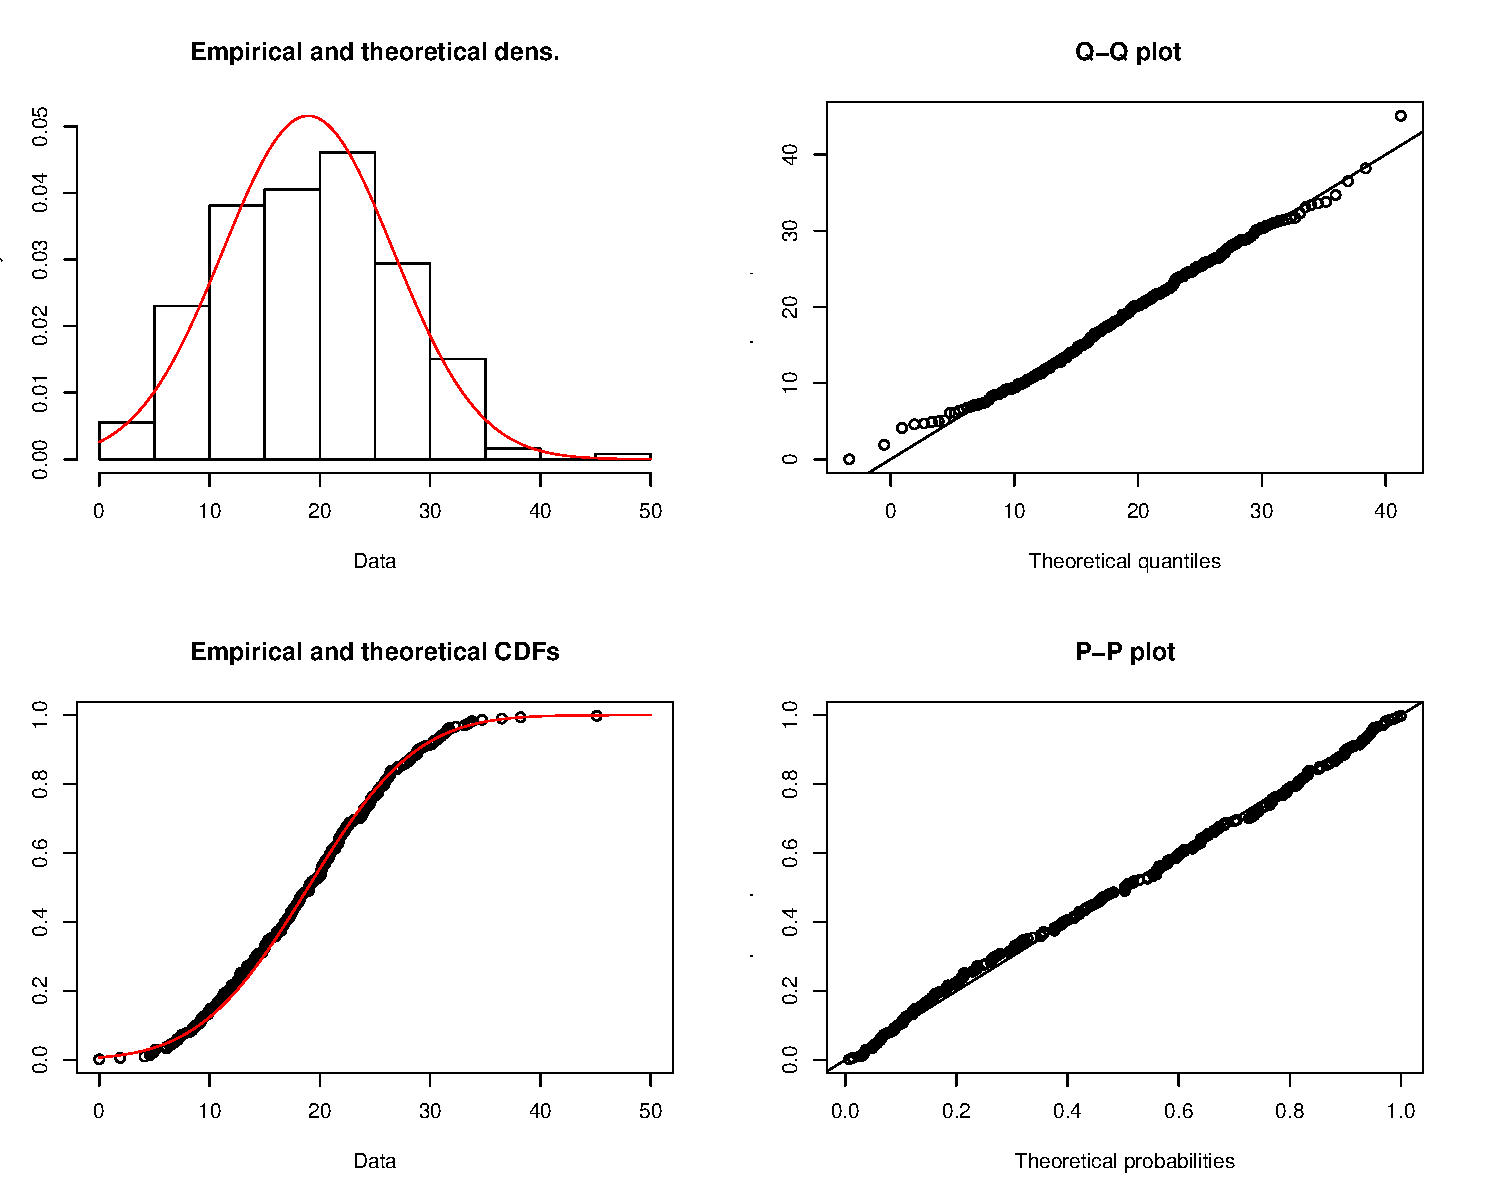
\includegraphics[width=0.8\linewidth]{Images/FIGURES/brozek_fitdist}
	\caption{Normal distribution fit to fat percentage given by Brozek's equation.}
	\label{fig:brozek_fitdist}
\end{figure}
\vspace*{\fill}

\newpage


\subsection{Total Body Weight Scatter Plots}\label{sec:total_weight}

In this section we will look at the behavior of total body weight in the scope of the provided dataset. In Fig.~\ref{fig:total_weight_vs_density} a scatter plot against the body density can be seen. Once again our speculation about the fact, that the body density is decreasing with increasing body weight, is supported. Moreover, as we can see, the main reason for that is the increasing amount of fat. 

\medskip

Regarding the distribution of the total body weight, it is not a trivial task to perform a fit in this case. As one can see, both gamma (Fig.~\ref{fig:total_weight_gamma_fitdist}) and normal (Fig.~\ref{fig:total_weight_normal_fitdist}) distributions seem to be able to describe the variable relatively well. To determine the true distribution a number of statistical tests, which are available in section \ref{sec:analysis}, have to be carried out.

\bigskip

%\begin{figure}[H]
%	\centering
%	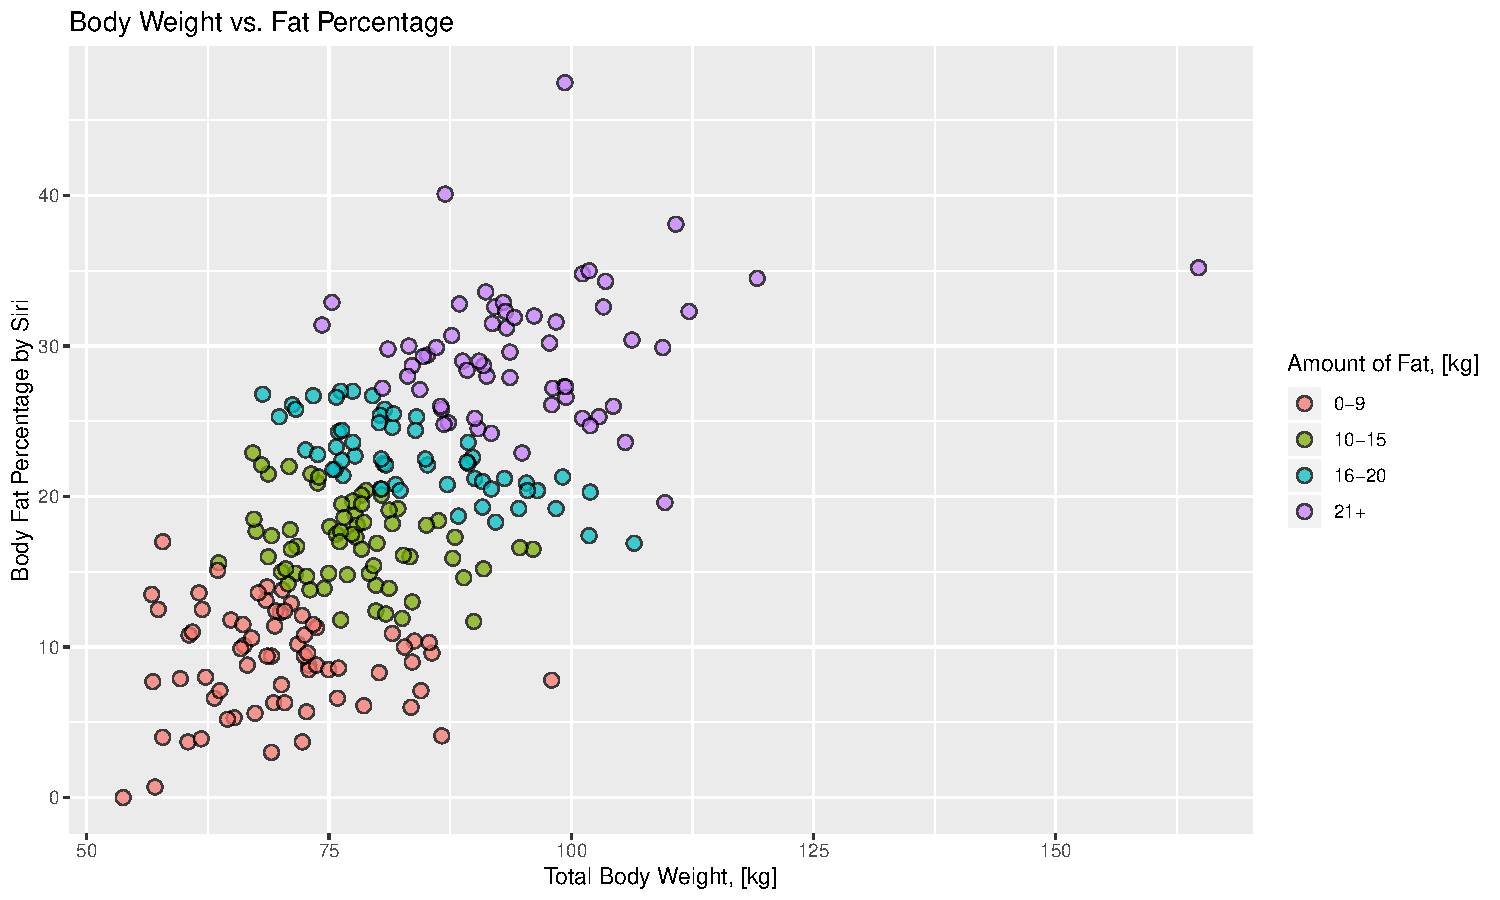
\includegraphics[width=1.0\linewidth]{Images/FIGURES/total_weight_vs_siri}
%	\caption{Influence of total body weight on the body fat percentage.}
%	\label{fig:total_weight_vs_siri}
%\end{figure}

\begin{figure}[H]
	\centering
	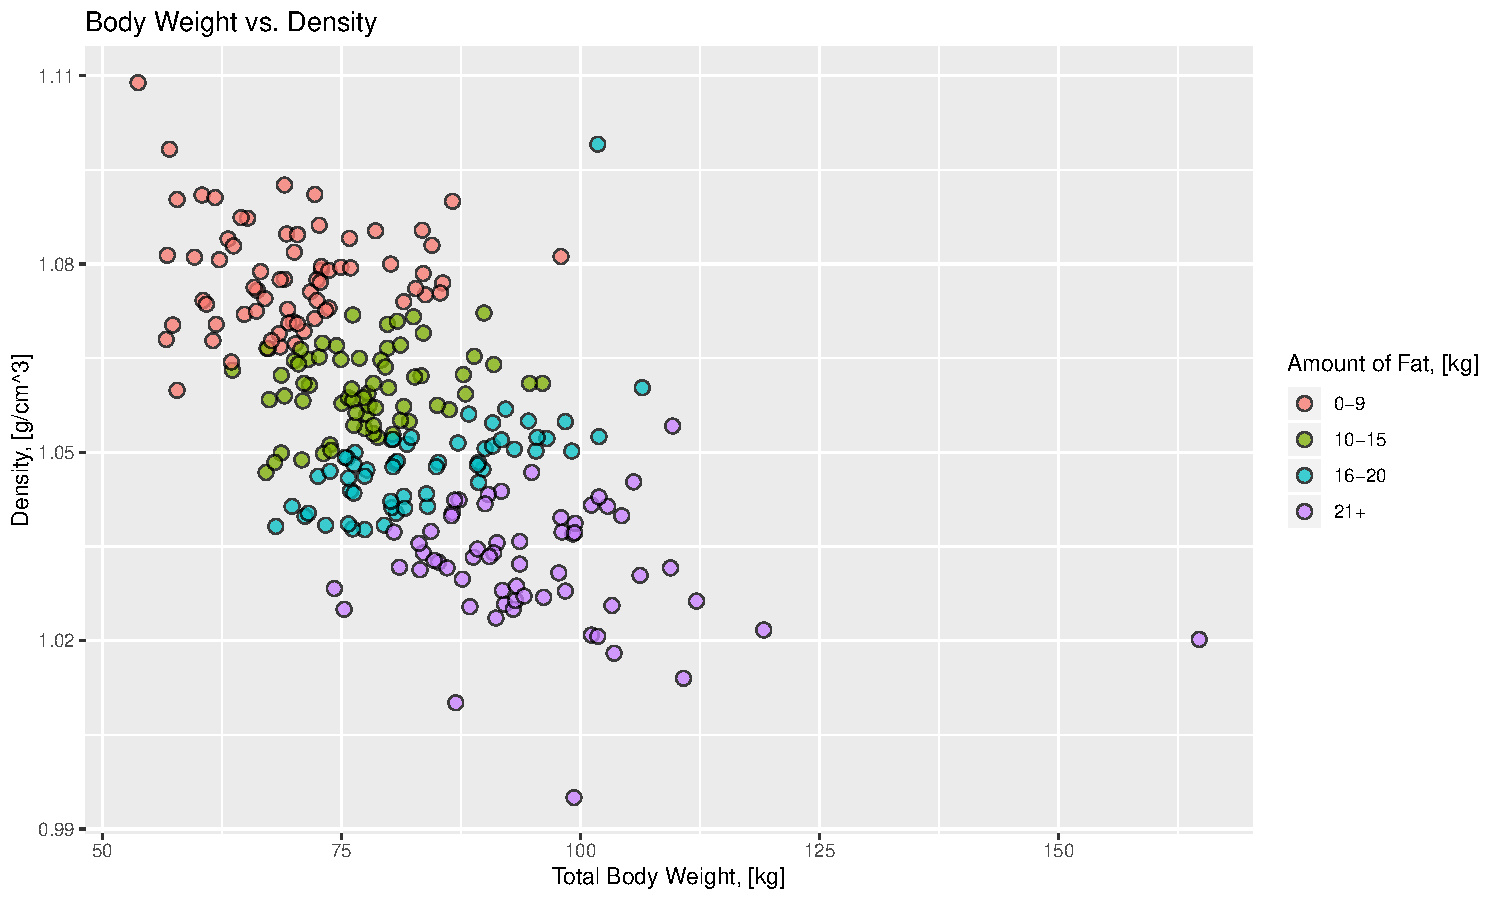
\includegraphics[width=1.0\linewidth]{Images/FIGURES/total_weight_vs_density}
	\caption{Influence of the total body weight on the body density.}
	\label{fig:total_weight_vs_density}
\end{figure}
\vspace*{\fill}

\newpage

\vspace*{\fill}
\begin{figure}[H]
	\centering
	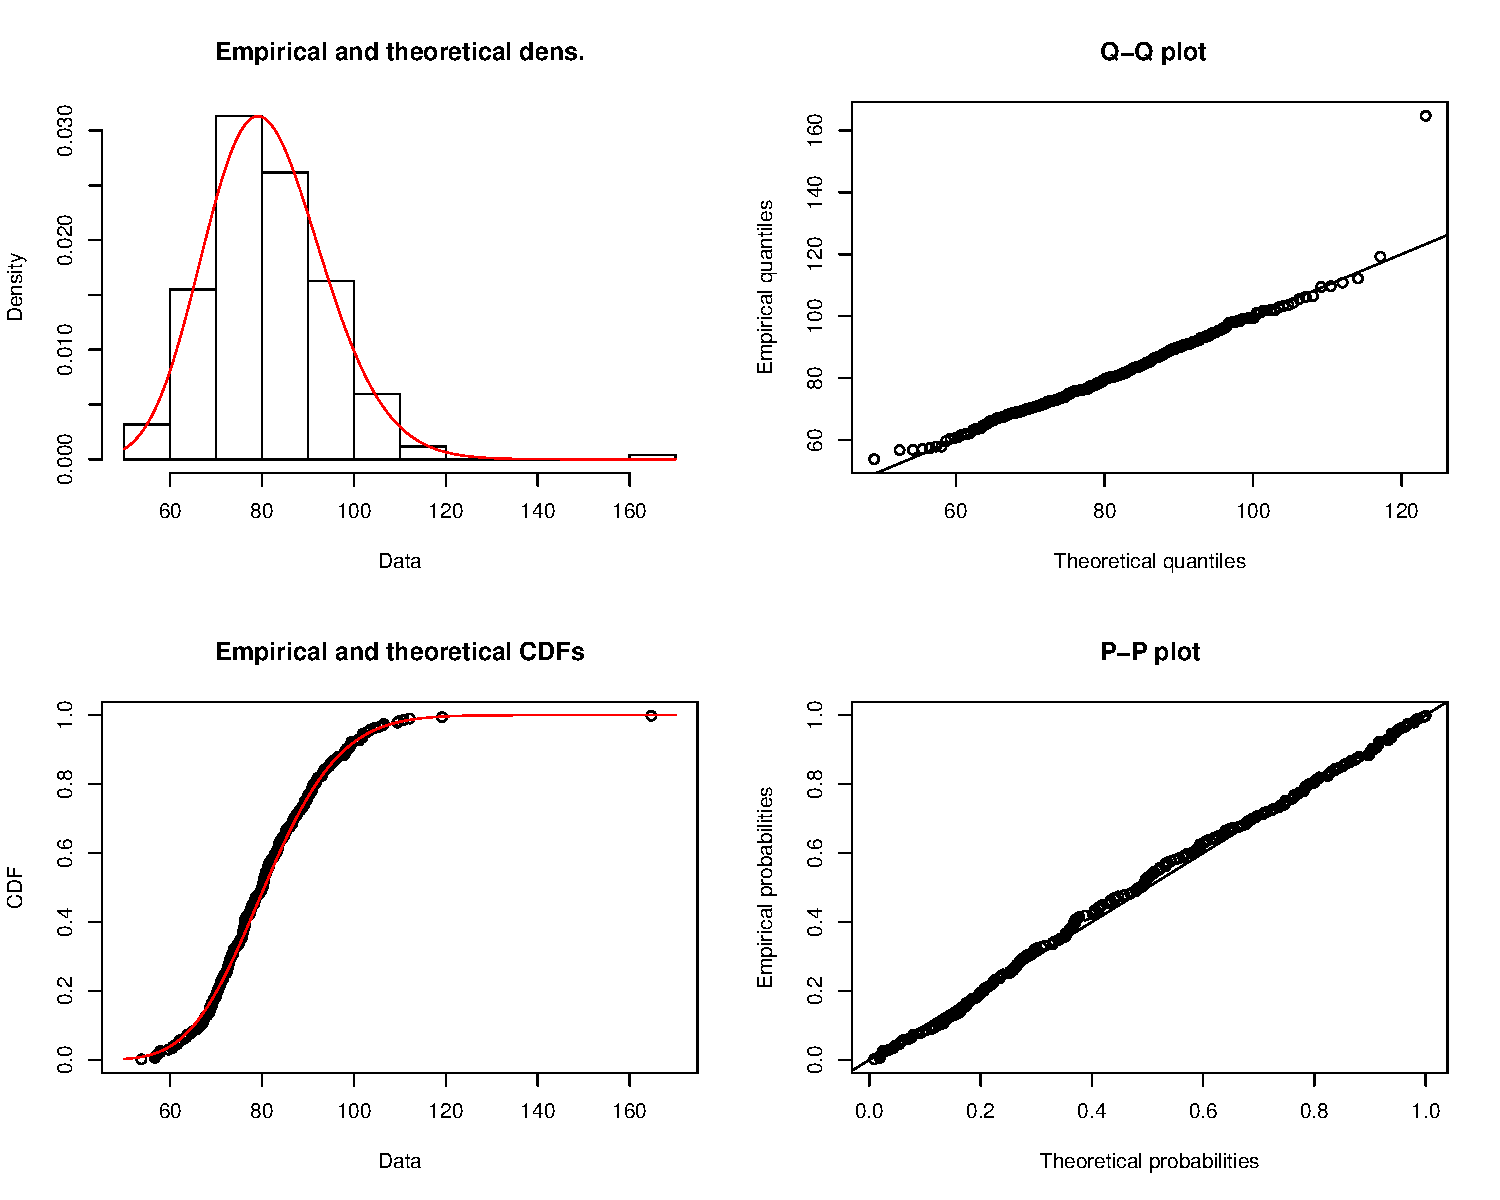
\includegraphics[width=0.8\linewidth]{Images/FIGURES/total_weight_gamma_fitdist}
	\caption{Gamma distribution fit to the total weight.}
	\label{fig:total_weight_gamma_fitdist}
\end{figure}

\begin{figure}[H]
	\centering
	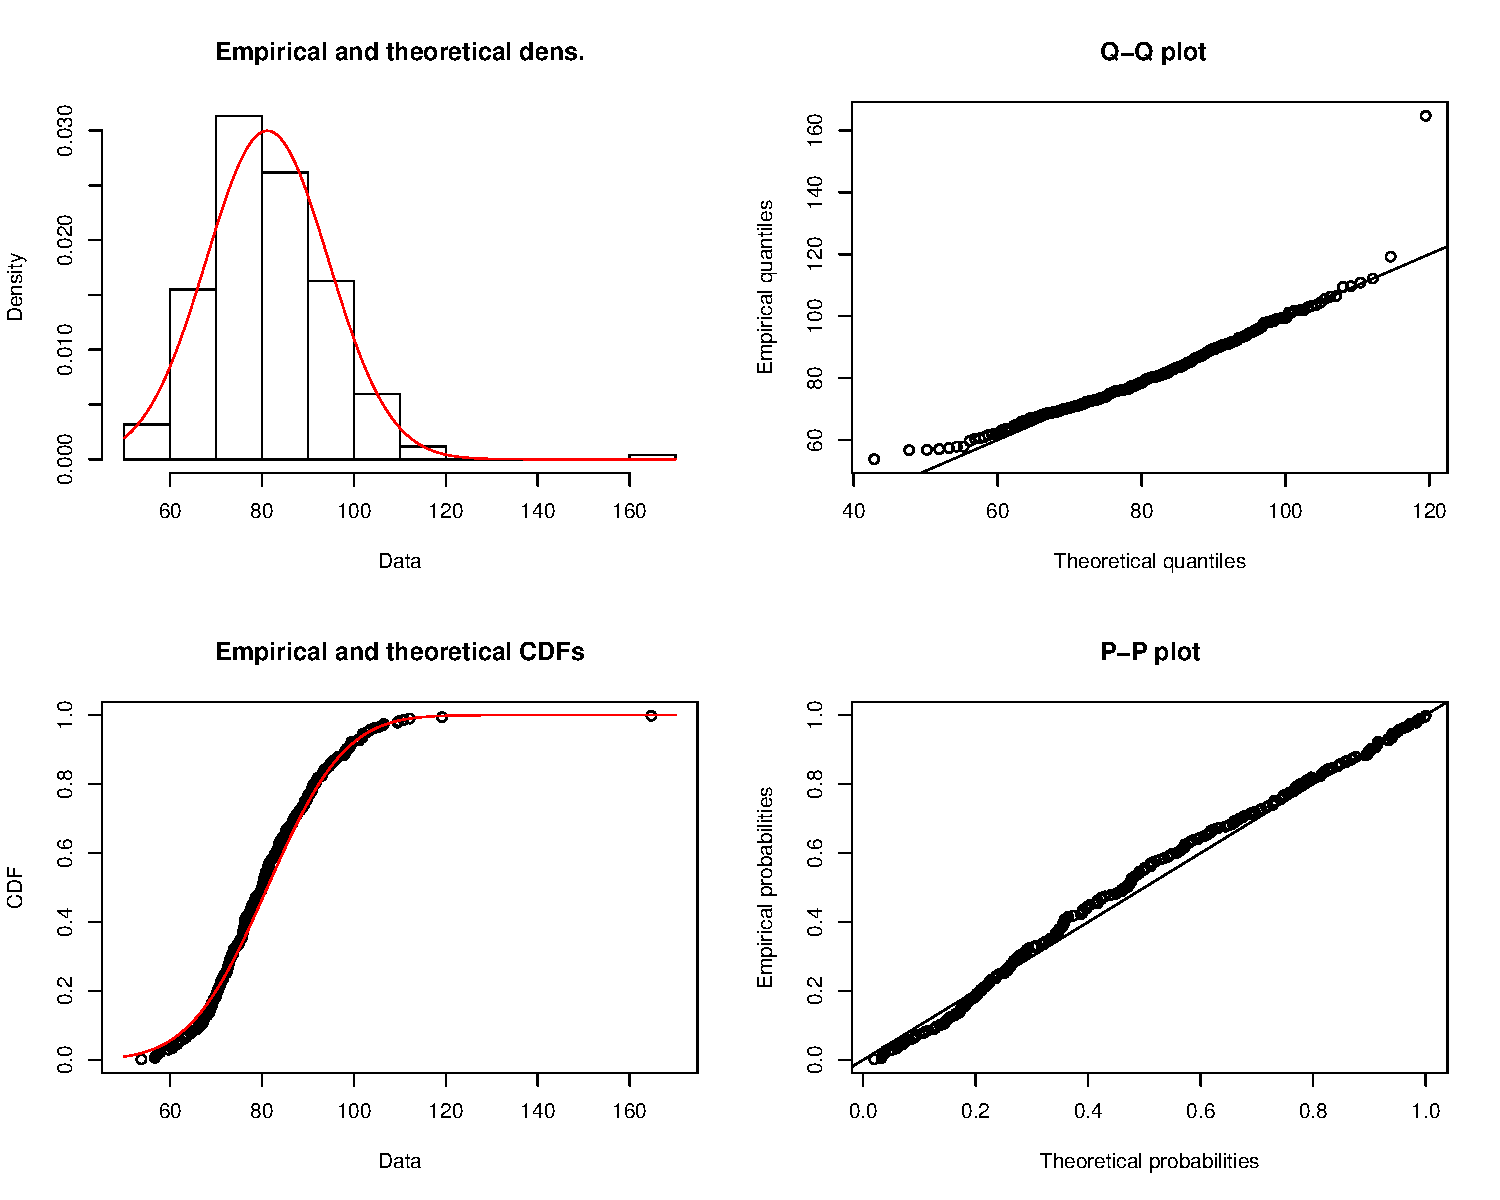
\includegraphics[width=0.8\linewidth]{Images/FIGURES/total_weight_normal_fitdist}
	\caption{Normal distribution fit to the total weight.}
	\label{fig:total_weight_normal_fitdist}
\end{figure}
\vspace*{\fill}

%\newpage
%
%\begin{figure}[H]
%	\centering
%	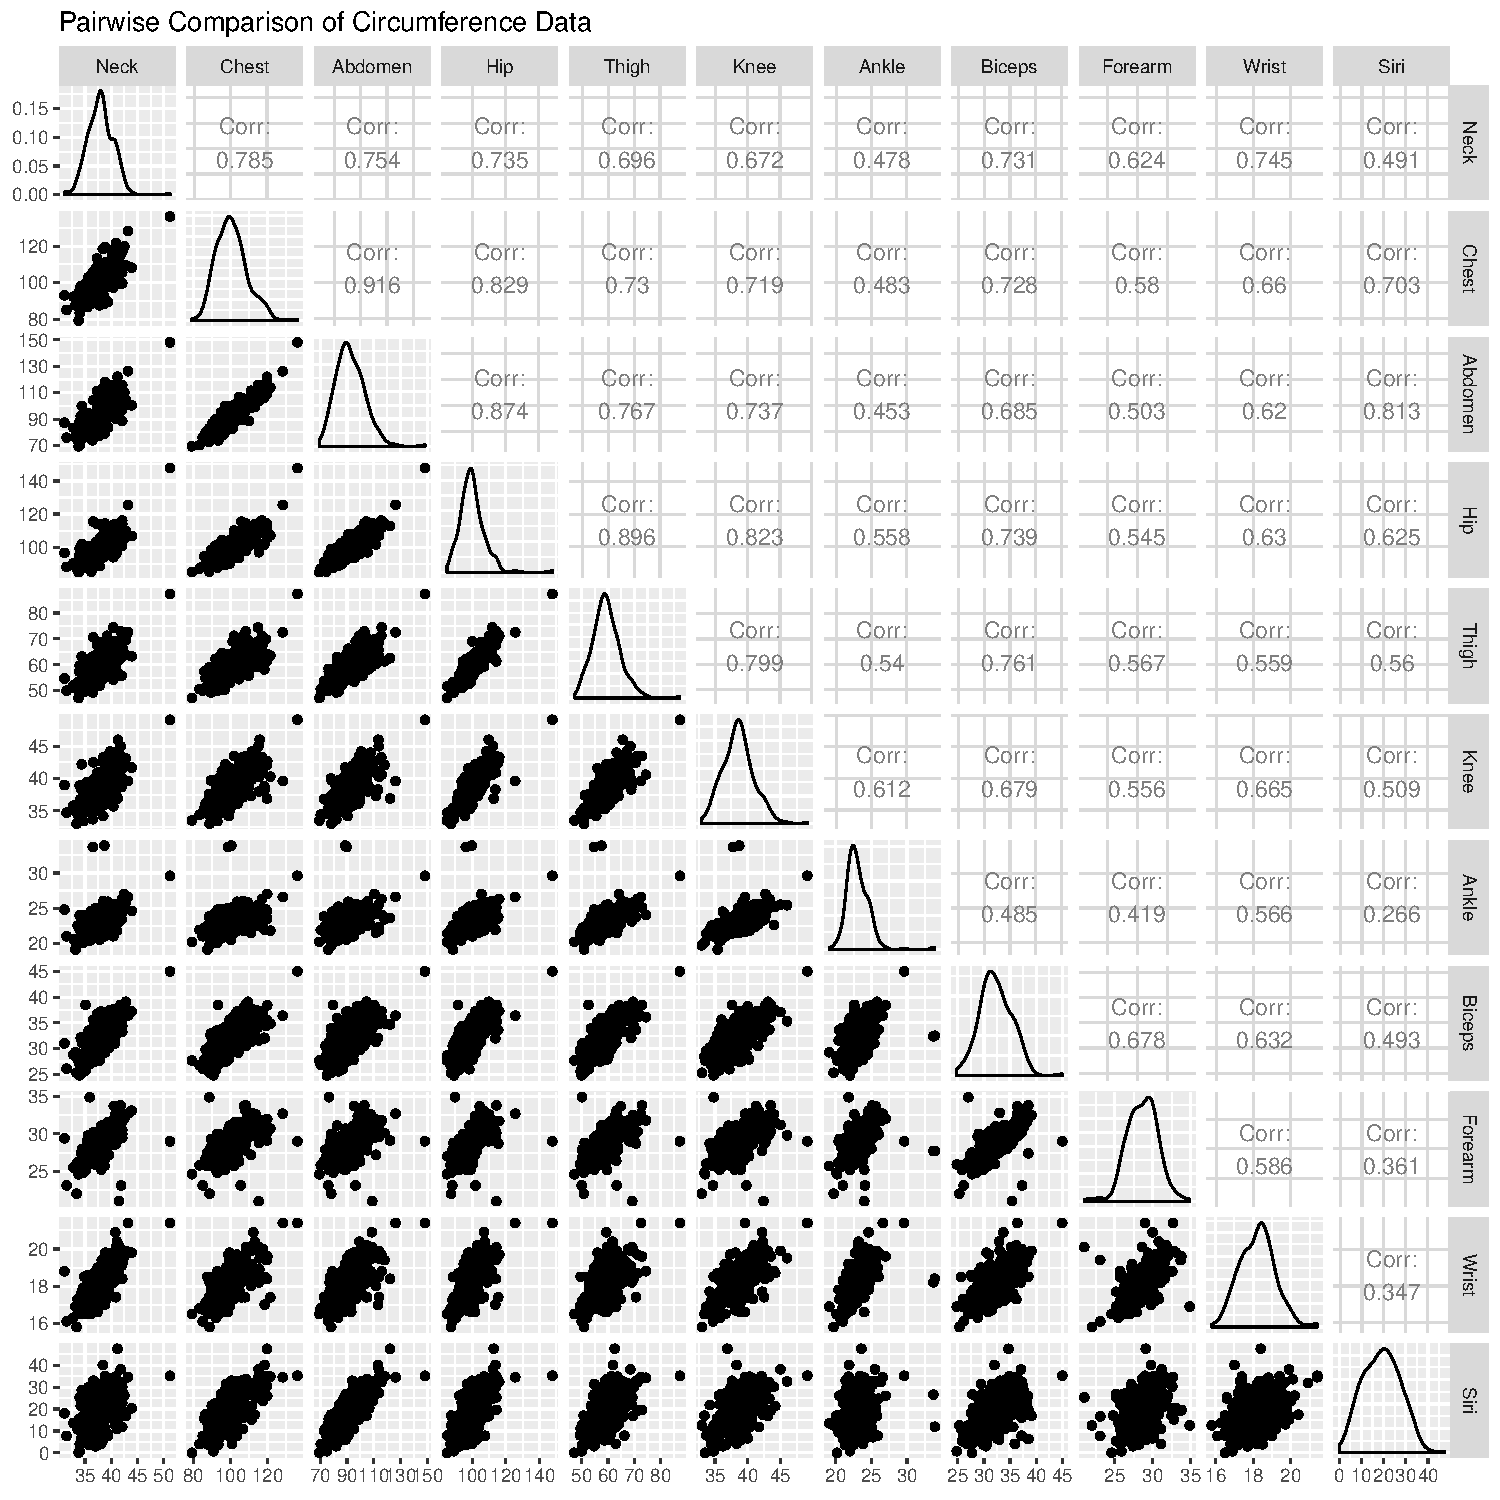
\includegraphics[width=1.0\linewidth]{Images/FIGURES/pairwise_comparison}
%	\caption{}
%	\label{fig:pairwise_comparison}
%\end{figure}


\newpage


\section{Data Analysis}\label{sec:analysis}

\textbf{Note:} all tests are performed with statistical significance $\alpha = 5\%$.

\subsection{Body Density Distribution}\label{sec:density_distr}

In the previous section we have performed a fit of normal distribution to the body density, and, according to presented diagrams, it seemed to be a reasonable thing to do. In this section a number of normality tests will be performed to support our hypothesis. Lilliefors and Shapiro-Wilk normality tests will be of aid: 

\begin{equation*}
	\text{H}_{0}: density \in \{ \mathcal{N} (\mu,\,\sigma^{2}): \mu \in \mathbb{R}, \, \sigma^{2} > 0 \} \text{ vs. }
	\text{H}_{1}: density \not\in \{ \mathcal{N} (\mu,\,\sigma^{2}): \mu \in \mathbb{R}, \, \sigma^{2} > 0 \}.
\end{equation*}

\medskip

Results of tests are displayed in the table below:

\begin{table*}[ht!]
	\centering
	\begin{tabular}{|c||c|c|}
		\hline 
		Name of the Test & Value of the Statistic & p-valiue \\ 
		\hline \hline
		Lilliefors & 0.038407 & 0.4864 \\ 
		\hline 
		Shapiro-Wilk & 0.9954 & 0.6571 \\ 
		\hline 
	\end{tabular} 
\end{table*}

According to both of the performed tests, no evidence against the null hypothesis is present. This entitles us to perform a normal distribution fit and perform the parametric Kolmogorov-Smirnov test (KS-test) to confirm, that the fitted distribution is the true one:

\begin{equation*}
	\text{H}_{0}: density = \mathcal{N} (\mu_{d},\,\sigma^{\,2}_{d}) \text{ vs. }
	\text{H}_{1}: density \neq \mathcal{N} (\mu_{d},\,\sigma^{\,2}_{d}).
\end{equation*}

\medskip

Estimated parameters of the normal distribution, their confidence intervals and results of the KS-test are available below:

\begin{table*}[ht!]
	\centering
	\begin{tabular}{|c||c||c|c||c|}
		\hline 
		Parameter &  Estimated Value & \multicolumn{2}{c||}{Confidence Interval, $95\%$}  & KS-test p-value \\ 
		\hline \hline 
		Mean, $\mu_{d}$ & 1.055574 & 1.053229 &  1.057919 & \multirow{2}{*}{0.8413} \\ 
		\cline{1-4}
		Standard Deviation, $\sigma_{d}$ & 0.018994 & 0.017356 &  0.020631 & \\ 
		\hline
	\end{tabular} 
\end{table*}

Once again we cannot reject the null hypothesis, and the distribution of the body density is truly $\mathcal{N} (\mu_{d},\,\sigma^{\,2}_{d})$.

\subsection{Analysis of Body Fat Percentage by Siri's and Brozek's Equations}

\subsubsection{Normality Tests}

In this section we will perform normality tests for fat percentage given by Siri's and Brozek's equations in the same manner as in section \ref{sec:density_distr}. The results of Lilliefors and Shapiro-Wilk tests are as follows:

\begin{table*}[ht!]
	\centering
	\begin{tabular}{|c||c||c|c|}
		\hline 
		Variable & Name of the Test & Value of the Statistic & p-valiue \\ 
		\hline \hline
		\multirow{2}{*}{Siri} & Lilliefors & 0.044548 & 0.2584 \\ 
		\cline{2-4} 
		 & Shapiro-Wilk & 0.99168 & 0.1649 \\ 
		\hline \hline
		\multirow{2}{*}{Brozek} & Lilliefors & 0.039781 & 0.429 \\ 
		\cline{2-4} 
		& Shapiro-Wilk & 0.99292 & 0.2747 \\ 
		\hline
	\end{tabular} 
\end{table*}

Tests entitle us to conclude, that the null hypothesis (normality of the distribution) cannot be rejected for both Siri's and Brozek's fat percentage. This enables us to proceed to KS-test:

\begin{table*}[ht!]
	\centering
	\begin{tabular}{|c||c||c||c|c||c|}
		\hline 
		Variable & Parameter &  Estimated Value & \multicolumn{2}{c||}{Confidence Interval, $95\%$}  & KS-test p-value \\ 
		\hline \hline 
		\multirow{2}{*}{Siri} & Mean, $\mu_{s}$ & 19.150794 & 18.119590 &  20.182 & \multirow{2}{*}{0.2159} \\ 
		\cline{2-5}
		& Standard Deviation, $\sigma_{s}$ & 8.352119 & 7.622948 &  9.08129 & \\ 
		\hline \hline
		\multirow{2}{*}{Brozek} & Mean, $\mu_{b}$ & 18.938492 & 17.983425 &  19.893560 & \multirow{2}{*}{0.8193} \\ 
		\cline{2-5}
		& Standard Deviation, $\sigma_{b}$ & 7.735462 & 7.060127 &  8.410796 & \\ 
		\hline
	\end{tabular} 
\end{table*}

P-values allow us to conclude, that fat percentage given by both Siri's and Brozek's equations is normally distributed ($\mathcal{N} (\mu_{s},\,\sigma^{\,2}_{s})$ and $\mathcal{N} (\mu_{b},\,\sigma^{\,2}_{b})$, respectively).

\subsubsection{Equality of Distributions}

In this section we will perform the unpaired two-sample Kolmogorov-Smirnov test to determine, if distributions of fat percentage given by Siri's and Brozek's equations are equal. From the comparative diagram of cumulative distribution functions (Fig.~\ref{fig:cdf_brozek_siri}) it is obvious, that no significant horizontal shifts are present. Thus, the KS-test will provide a sufficient and reliable result:

\begin{equation*}
	\text{H}_{0}: F=G \text{ vs. }
	\text{H}_{1}: F \neq G
\end{equation*}

\medskip
\noindent
where $F$ and $G$ are distribution functions of fat percentage calculated using Siri's and Brozek's equations, respectively.\footnote{We already know, that those distributions are normal, and their parameters have already been estimated. However, the unpaired two-sample KS-test is nonparametric.} Results of the test are positive, as the p-value is equal to $0.9375$ which means, that no strong evidence against the null hypothesis is existent - distributions are similar.\footnote{The unpaired two-sample Wilcoxon test works well to detect horizontal shifts in compared CDFs. We did not use this test to reach the conclusion, however, its results are also positive: p-value$\,=0.7789$.}

\subsection{Total Weight Distribution}

In the scope of this section the distribution of the total weight of the population will be determined. As seen in section \ref{sec:total_weight} we are unable to determine which distribution fits to the total weight better: gamma or normal. Taking a closer look at the Q-Q plot (Fig.~\ref{fig:qq_total_weight}) gives us a clue, that fitting with gamma distribution appears to be slightly more competent.\footnote{The point at the top-right part of both diagrams is an obvious outlier.} 

\begin{figure}[H]
	\centering
	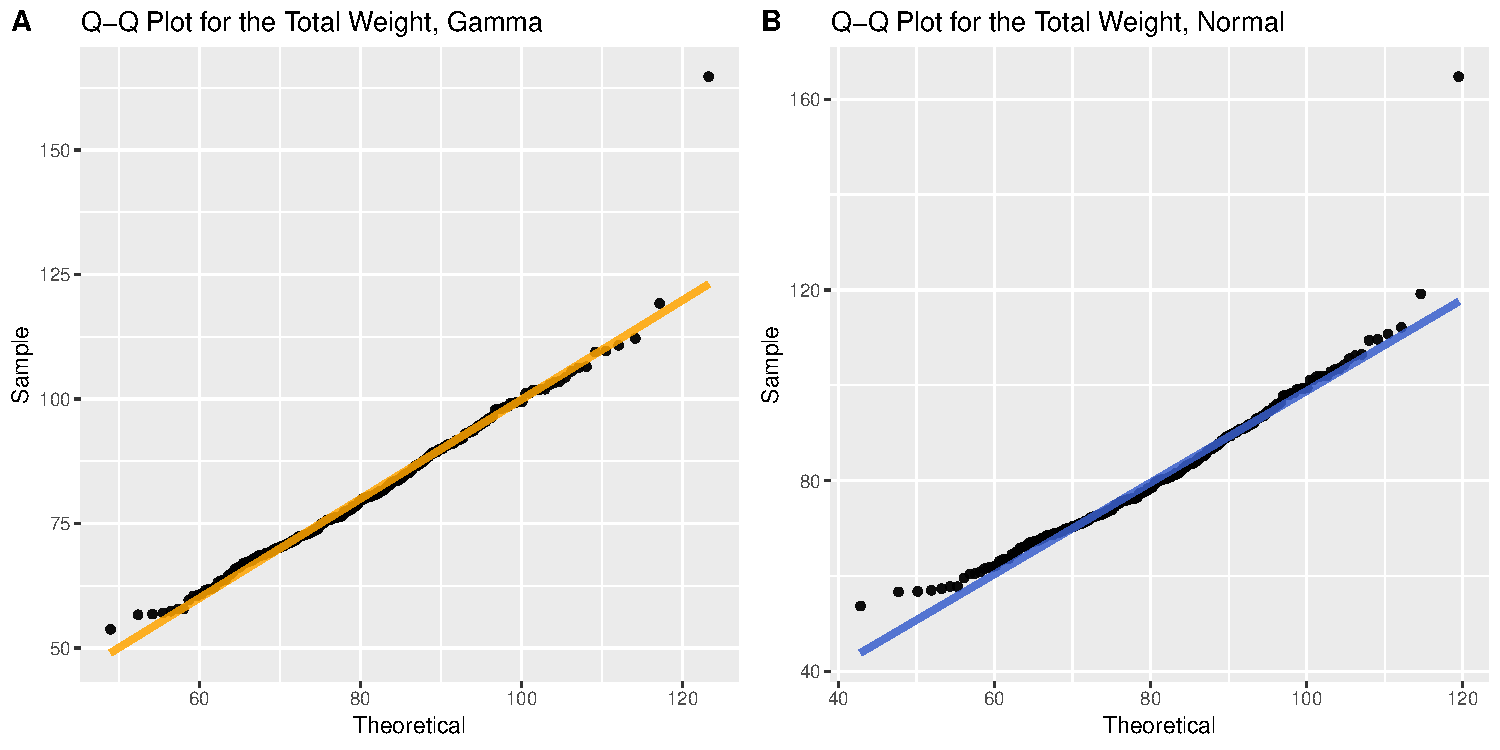
\includegraphics[width=0.9\linewidth]{Images/FIGURES/qq_total_weight}
	\caption{Q-Q plot for estimated Gamma and Normal distributions for the total weight.}
	\label{fig:qq_total_weight}
\end{figure}

However, we will test both distributions using Chi-squared and Kolmogorov-Smirnov tests:

\begin{equation*}
\text{H}_{0}^{(G)}: weight = Gamma(\alpha_{w}, \, \beta_{w}) \text{ vs. }
\text{H}_{1}^{(G)}: weight \neq Gamma(\alpha_{w}, \, \beta_{w}),
\end{equation*}
\begin{equation*}
\text{H}_{0}^{(N)}: weight = \mathcal{N} (\mu_{w},\,\sigma^{\,2}_{w}) \text{ vs. }
\text{H}_{1}^{(N)}: weight \neq \mathcal{N} (\mu_{w},\,\sigma^{\,2}_{w}).
\end{equation*}

\begin{table*}[ht!]
	\centering
	\begin{tabular}{|c||c||c|c|}
		\hline 
		Tested Distribution & Name of the Test & Value of the Statistic & p-valiue \\ 
		\hline \hline
		\multirow{2}{*}{Gamma} & Chi-squared & 2.9615 & 0.9975 \\ 
		\cline{2-4} 
		& Kolmogorov-Smirnov & 0.039134 & 0.835 \\ 
		\hline \hline
		\multirow{2}{*}{Normal} & Chi-squared & 7.3248 & 0.8881 \\ 
		\cline{2-4} 
		& Kolmogorov-Smirnov & 0.060868 & 0.308 \\ 
		\hline
	\end{tabular} 
\end{table*}

P-values of tests do not suggest to reject either $\text{H}_{0}^{(G)}$ or $\text{H}_{0}^{(N)}$. On the other hand, they favor gamma distribution (especially, KS-test: p-value$^{(G)}$ is greater than p-value$^{(N)}$ by $0.527$). That is the main reason behind us choosing gamma distribution as the best fit to the total weight of the population. In the table below estimated values of distribution parameters are displayed:

\begin{table*}[ht!]
	\centering
	\begin{tabular}{|c||c||c|c|}
		\hline 
		Parameter &  Estimated Value & \multicolumn{2}{c|}{Confidence Interval, $95\%$}  \\ 
		\hline \hline 
		Shape, $\alpha_{w}$ & 39.731517 & 32.824526 &  46.638507 \\ 
		\cline{1-4}
		Scale, $\beta_{w}$ & 0.489557 & 0.403914 &  0.575201 \\ 
		\hline
	\end{tabular} 
\end{table*}

To sum up, we have statistically proved, that the distribution of the total weight within the population is $Gamma(\alpha_{w}, \, \beta_{w})$.


\section{Multivariate Linear Regression}\label{sec:regression}

In the scope of this section we will consider observation $39$ with total weight equal to $164.7$ kg as an outlier and remove it from the dataset.

\subsection{Two-variable Linear Regression}

In this section we will assume, that the results of Siri's equation can be explained by two variables: abdomen circumference and total weight. Then the linear model takes the following form, $\forall i \in \{1,2, \dots, 251\}$:

\begin{equation}
		Y_{i} = \beta_{0} + \beta_{1} X_{i,\,1} + \beta_{2} X_{i,\,2} + e_{i}
\end{equation}

\medskip
\noindent
which, with dropped mathematical notation for the response and explanatory variables, results in

\begin{equation*}
	\text{(Body Fat Percentage by Siri)} = \beta_{0} + \beta_{1} \cdot (\text{Abdomen CC}) + \beta_{2} \cdot (\text{Total Weight}).
\end{equation*}

\medskip

Results of the estimation can be observed in the table below. The value of the R-squared statistic is equal to $0.72$. This indicates, that $72\%$ of the variability of the response data is explained around its mean which is quite adequate for our purposes. 

\begin{table}[H]
	\centering
	\begin{tabular}{|c||c||c|c|}
		\hline 
		Parameter &  Estimated Value & \multicolumn{2}{c|}{Confidence Interval, $95\%$}  \\ 
		\hline \hline 
		Intercept, $\beta_{0}$ & -47.67 & -52.86 &  -42.48 \\ 
		\hline 
		Abdomen CC, $\beta_{1}$ & 0.98 & 0.87 &  1.09 \\ 
		\hline 
		Total Weight, $\beta_{2}$ & -0.29 & -0.38 & -0.2 \\ 
		\hline 
	\end{tabular} 
\caption{Estimated values for the 2-variable linear regression.}
\end{table}

The fit is displayed in Fig.~\ref{fig:3d_linear_regression}. As can be seen in the Fig.~\ref{fig:2var_linear_regression}, the residuals are distributed acceptably on the plane (see the first column of the figure), normal Q-Q plot also indicates normality of residuals. Assuredly, as normality of residuals is the absolute assumption to perform linear regression, a relevant test has to be performed to support this hypothesis.

\begin{equation*}
	\text{H}_{0}: res \in \{ \mathcal{N} (\mu,\,\sigma^{2}): \mu \in \mathbb{R}, \, \sigma^{2} > 0 \} \text{ vs. }
	\text{H}_{1}: res \not\in \{ \mathcal{N} (\mu,\,\sigma^{2}): \mu \in \mathbb{R}, \, \sigma^{2} > 0 \}
\end{equation*}

\medskip

According to the Lilliefors test with statistical significance set to $5\%$ we cannot reject the null hypothesis, as the p-value is equal to $0.33$ - usage of the linear model is permitted.

\newpage

\vspace*{\fill}
\begin{figure}[H]
	\centering
	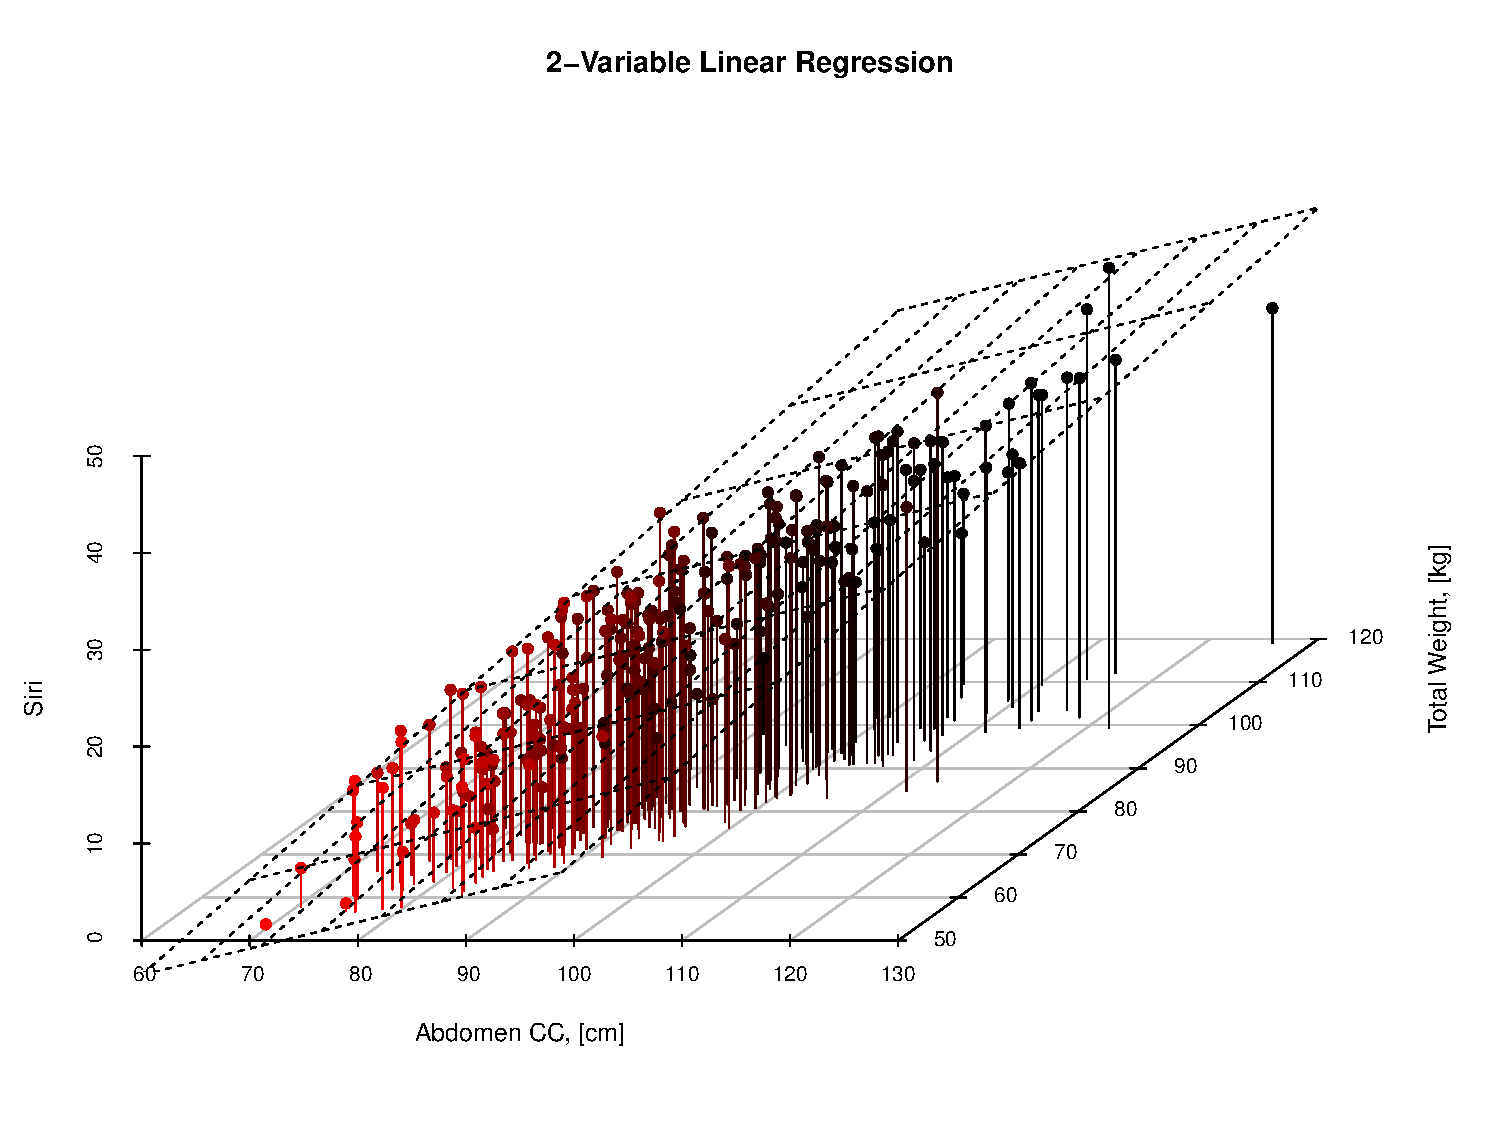
\includegraphics[width=0.75\linewidth]{Images/FIGURES/3d_linear_regression}
	\caption{Fit of the linear model with two explanatory variables.}
	\label{fig:3d_linear_regression}
\end{figure}

\begin{figure}[H]
	\centering
	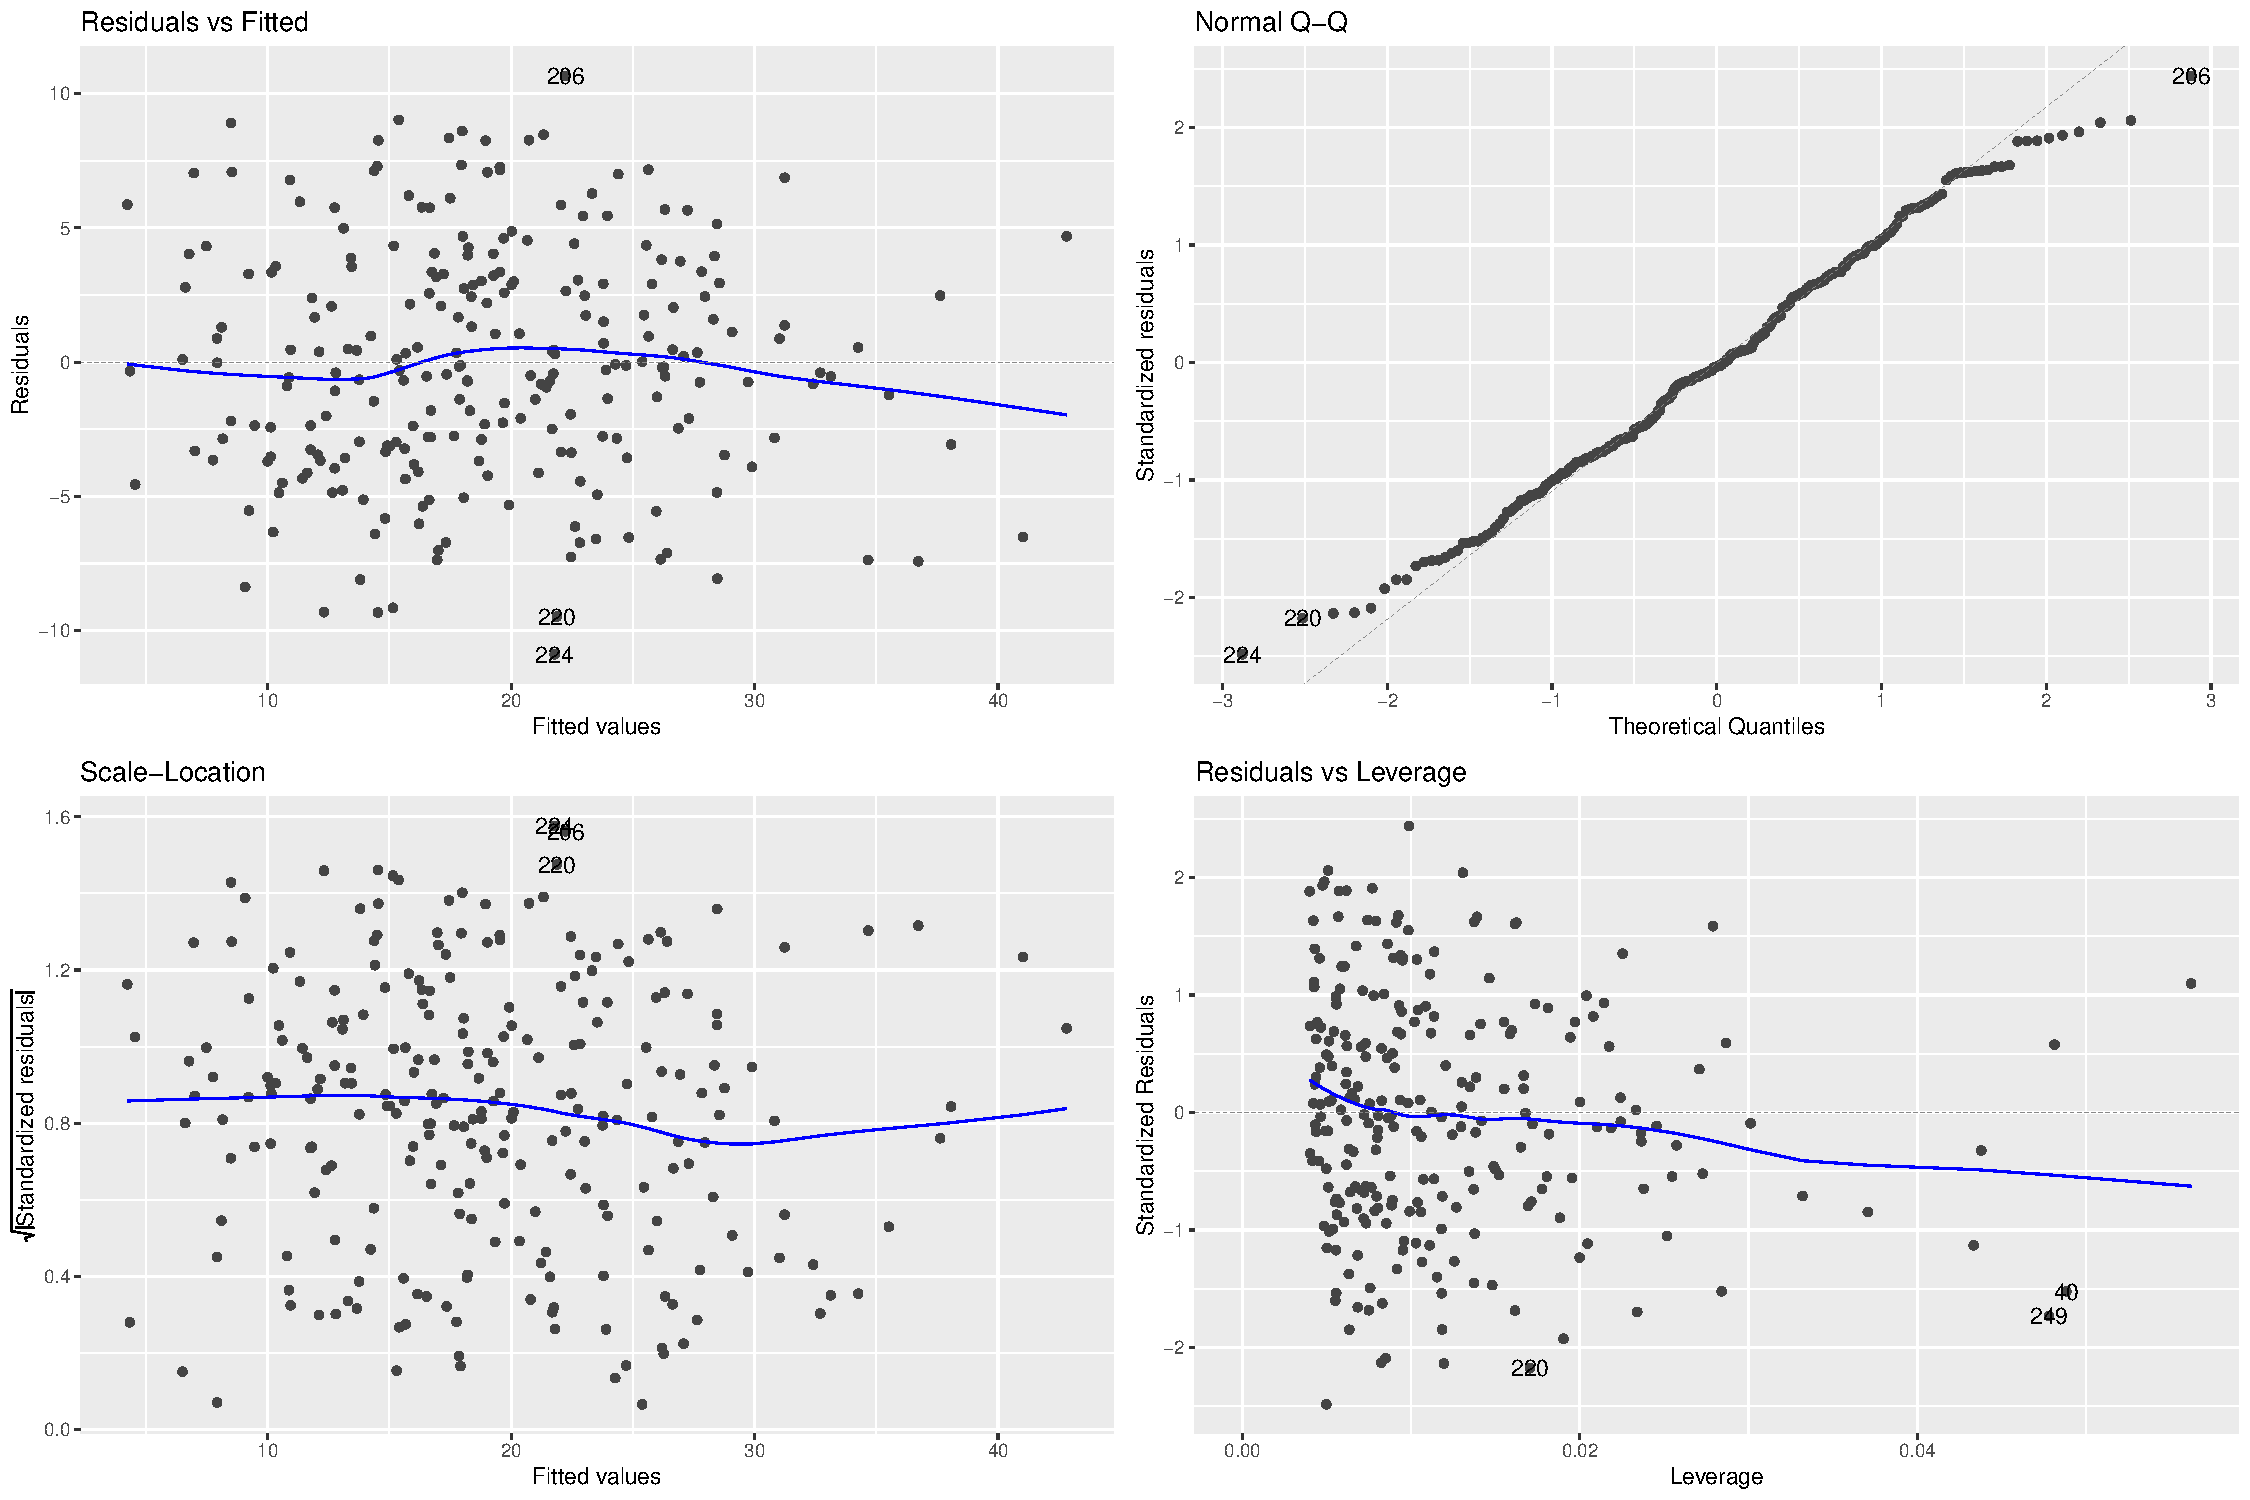
\includegraphics[width=0.95\linewidth]{Images/FIGURES/2var_linear_regression}
	\caption{Two-variable linear regression results diagram.}
	\label{fig:2var_linear_regression}
\end{figure}
\vspace*{\fill}

\newpage

\subsection{Multiple Linear Regression}

\subsubsection{All Variables Included}

Now we will consider the model with almost all available variables and once again attempt to explain the fat percentage given by Siri's equation. The model is as follows, $\forall i \in \{1,2, \dots, 251\}$:\footnote{In contrast with the previous section, we also exclude the intercept from the model from by reason of common sense: with decreasing values of explanatory variables the fat percentage also decreases.}

\begin{equation}
	Y_{i} = \sum_{j = 1}^{15}\beta_{j} X_{i,\,j} + e_{i}
\end{equation}

\medskip
\noindent
or $Y = X \beta + e$ in a matrix form. Estimated values are displayed in the Tab.~\ref{tab:multivar_regression}. The R-squared statistic is quite high for the observed model and is equal to $0.995$ which means, that almost all of the response data variability is explained. Nonetheless, a lot of confidence intervals for estimated parameters contain $0$. Moreover, residuals are not normally distributed (see Fig.~\ref{fig:multivar_linear_regression_all}), as the null hypothesis in the Lilliefors test is rejected due to the p-value equal to $5.101 \cdot 10^{-7}$. Thus, linear regression cannot be used for this set of explanatory variables.

\begin{table}[H]
	\centering
	\begin{tabular}{|c||c||c|c|}
		\hline 
		Parameter &  Estimated Value & \multicolumn{2}{c|}{Confidence Interval, $95\%$}  \\ 
		\hline \hline 
		Age, $\beta_{1}$ & 0.01 & -0.01 &  0.04 \\ 
		\hline 
		Total Weight, $\beta_{2}$ & 0.89 & 0.84 &  0.95 \\ 
		\hline 
		Height, $\beta_{3}$ & 0.01 & -0.01 & 0.04 \\ 
		\hline
		Adiposity, $\beta_{4}$ & -0.27 & -0.47 & -0.06  \\
		\hline 
		Fat-free weight, $\beta_{5}$ & -1.23 & -1.29 & -1.18  \\
		\hline
		Neck CC, $\beta_{6}$ & 0.05 & -0.1 & 0.2  \\
		\hline
		Chest CC, $\beta_{7}$ & 0.02 & -0.04 & 0.09  \\
		\hline
		Abdomen CC, $\beta_{8}$ & 0.1 & 0.03 & 0.18  \\
		\hline
		Hip CC, $\beta_{9}$ & -0.01 & -0.09 & 0.07  \\
		\hline
		Thigh CC, $\beta_{10}$ & 0.13 & 0.04 & 0.23  \\
		\hline
		Knee CC, $\beta_{11}$ & 0.05 & -0.1 & 0.21  \\
		\hline
		Ankle CC, $\beta_{12}$ & 0.12 & -0.02 & 0.26  \\
		\hline
		Biceps CC, $\beta_{13}$ & 0.12 & 0.01 & 0.23  \\
		\hline
		Forearm CC, $\beta_{14}$ & 0.08 & -0.05 & 0.22  \\
		\hline
		Wrist CC, $\beta_{15}$ & -0.07 & -0.42 & 0.28  \\
		\hline
	\end{tabular} 
	\caption{Estimated values for the multivariate linear regression with all parameters included.}
	\label{tab:multivar_regression}
\end{table}



\subsubsection{The Final Model}

To make regression sufficient and authorized to be used, we exclude the total weight from the model due to its strong correlation ($0.76$) with the fat-free weight and run a stepwise algorithm to choose the best model by the Akaike Information Criterion. After excluding variables with low significance, we construct the final linear model using only  $8$ columns of the provided dataset: age, adiposity, fat-free weight, abdomen CC, hip CC, knee CC, biceps CC and wrist CC. Estimates of parameters are available in Tab.~\ref{tab:multivar_regression_final}. Fortunately, the R-squared statistic has remained high: $R^{2} = 0.9766$, thus, almost all of the variability of the response variable is accounted for by our model.

\medskip

As can be seen, confidence intervals no longer contain zeros. As for residuals (see Fig.~\ref{fig:multivar_linear_regression_final}), their normality is evident. Moreover, the Lilliefors test with statistical significance set to $5\%$ has resulted in our inability to reject the null hypothesis, as the p-value is equal to $0.4$. Hence, residuals distribution may be considered normal and we are eligible to use this model to perform multivariate linear regression.

\newpage

\vspace*{\fill}
\begin{table}[ht!]
	\centering
	\begin{tabular}{|c||c||c|c|}
		\hline 
		Parameter &  Estimated Value & \multicolumn{2}{c|}{Confidence Interval, $95\%$}  \\ 
		\hline \hline 
		Age, $\beta_{1}$ & -0.05 & -0.09 &  -0.01 \\ 
		\hline 
		Adiposity, $\beta_{2}$ & 0.52 & 0.19 & 0.85  \\
		\hline 
		Fat-free weight, $\beta_{3}$ & -0.57 & -0.65 & -0.49  \\
		\hline
		Abdomen CC, $\beta_{4}$ & 0.72 & 0.6 & 0.84  \\
		\hline
		Hip CC, $\beta_{5}$ & -0.19 & -0.34 & -0.03  \\
		\hline
		Knee CC, $\beta_{6}$ & 0.34 & 0.02 & 0.66  \\
		\hline
		Biceps CC, $\beta_{7}$ & 0.38 & 0.16 & 0.61  \\
		\hline
		Wrist CC, $\beta_{8}$ & -1.54 & -2.13 & -0.95  \\
		\hline
	\end{tabular} 
	\caption{Estimated values for the multivariate linear regression in the final model.}
	\label{tab:multivar_regression_final}
\end{table}

\vspace*{\fill}

\begin{figure}[ht!]
	\centering
	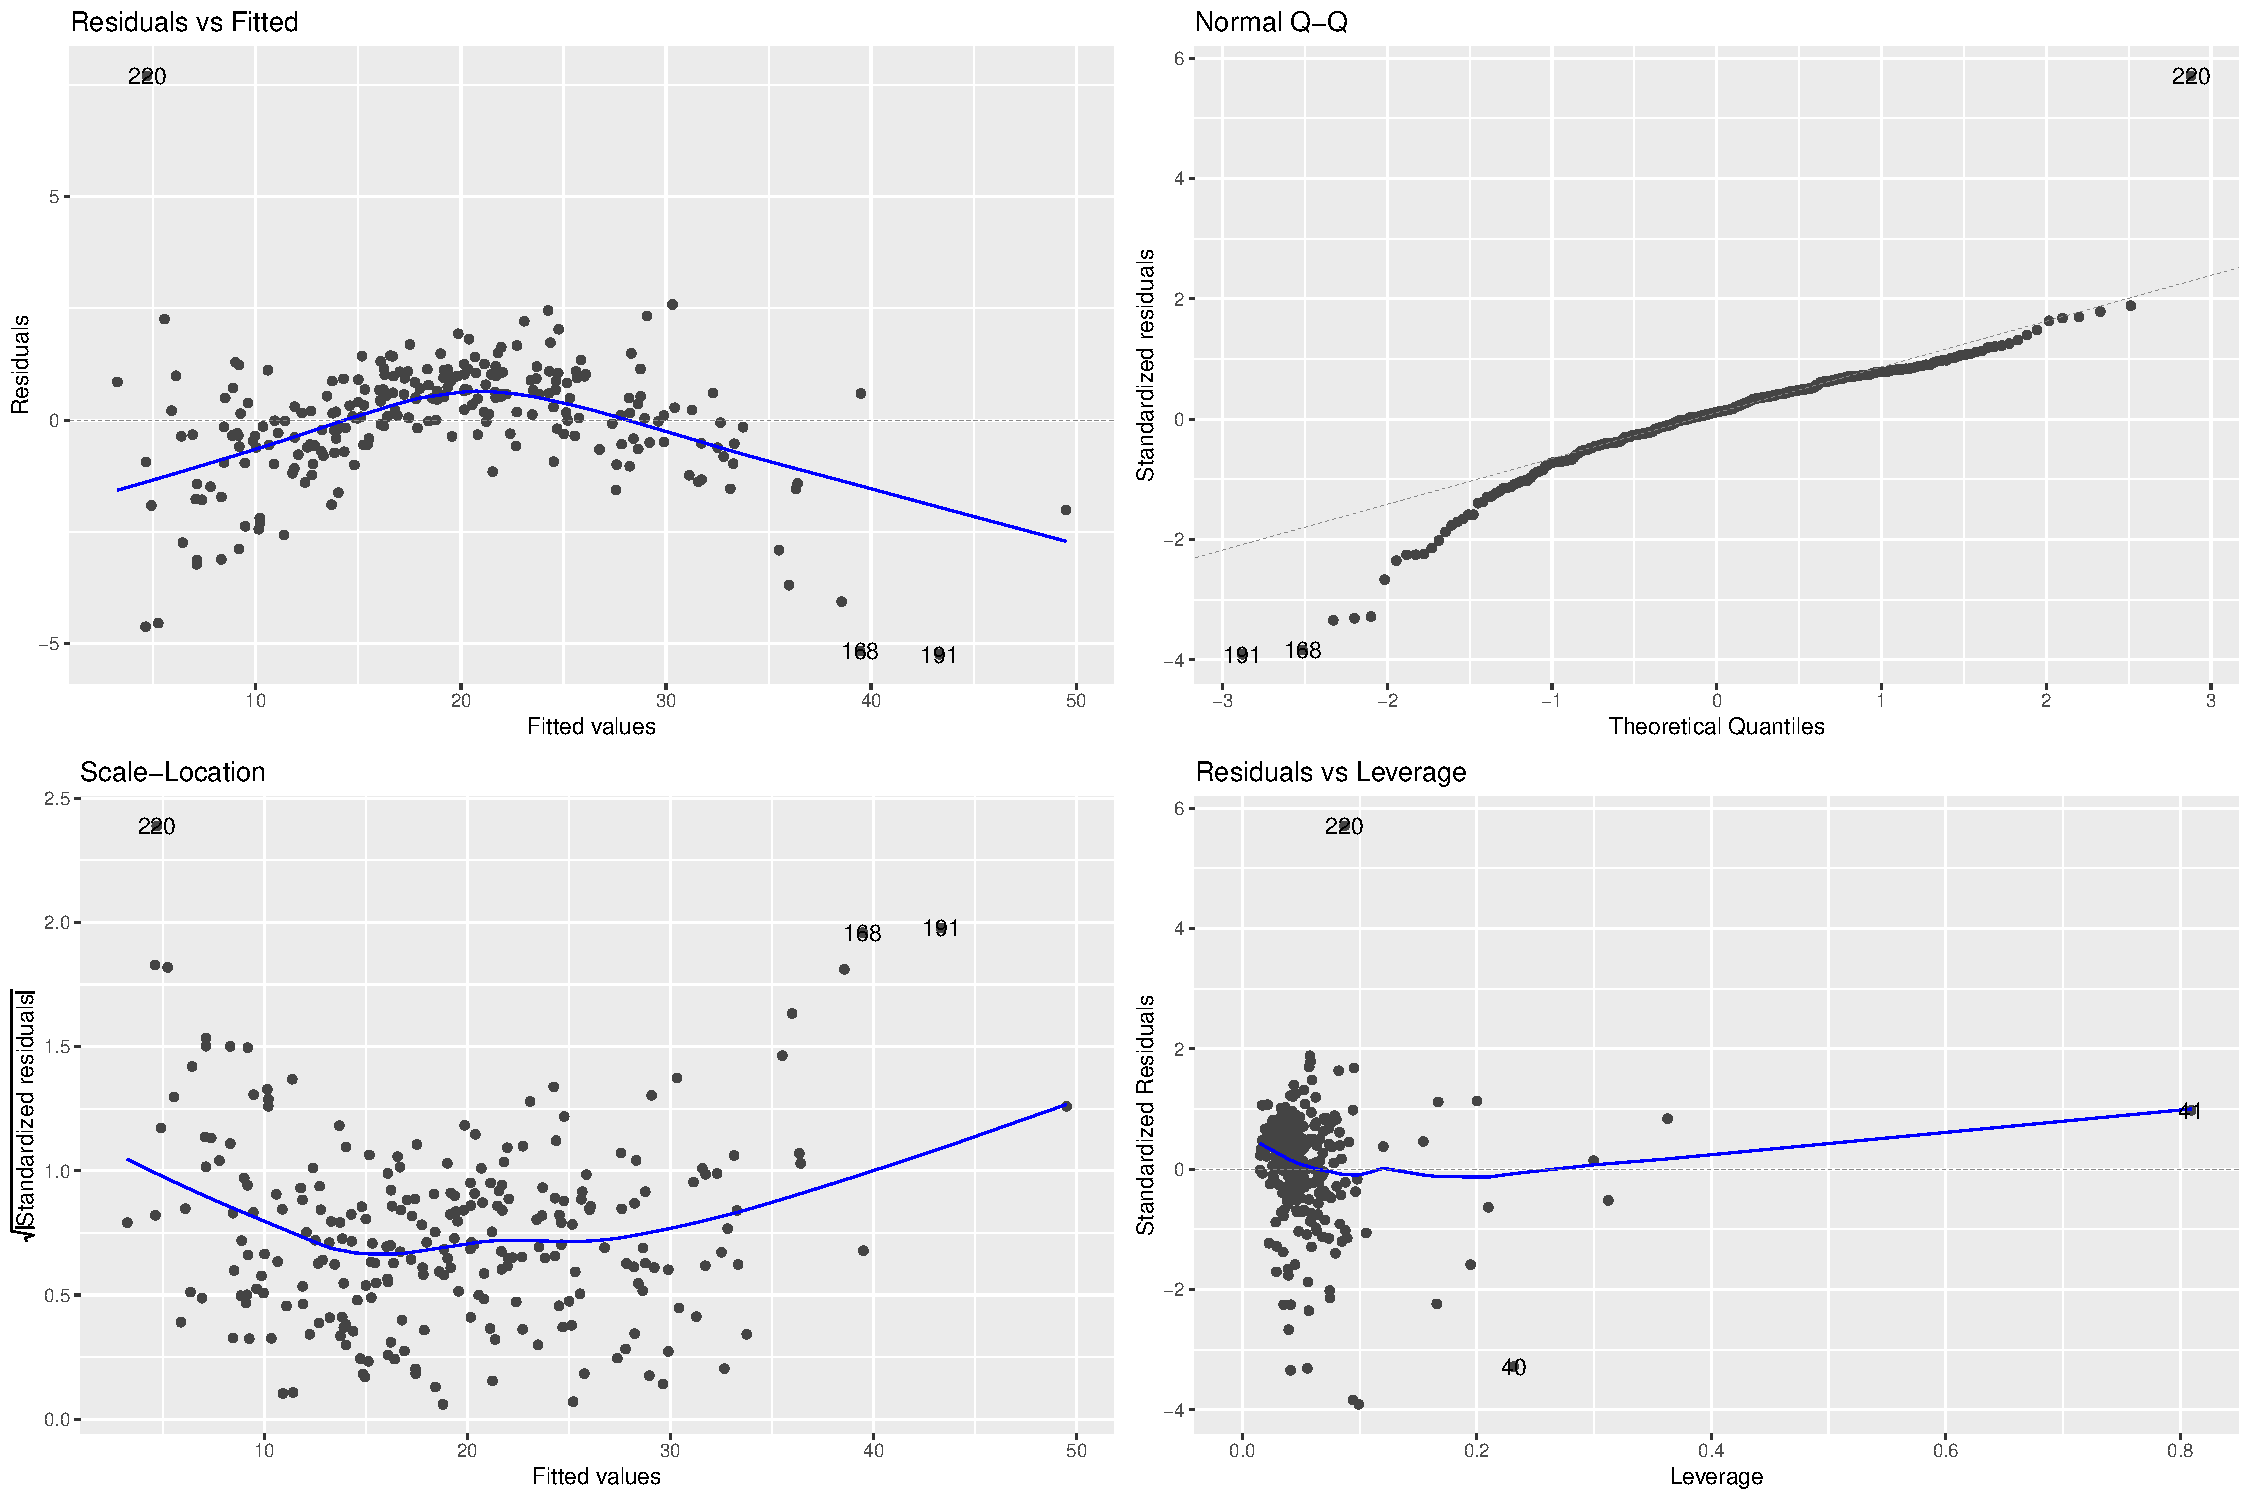
\includegraphics[width=0.95\linewidth]{Images/FIGURES/multivar_linear_regression_all}
	\caption{Multivariate linear regression results diagram for the model with all variables included.}
	\label{fig:multivar_linear_regression_all}
\end{figure}
\vspace*{\fill}

\newpage

\begin{figure}[ht!]
	\centering
	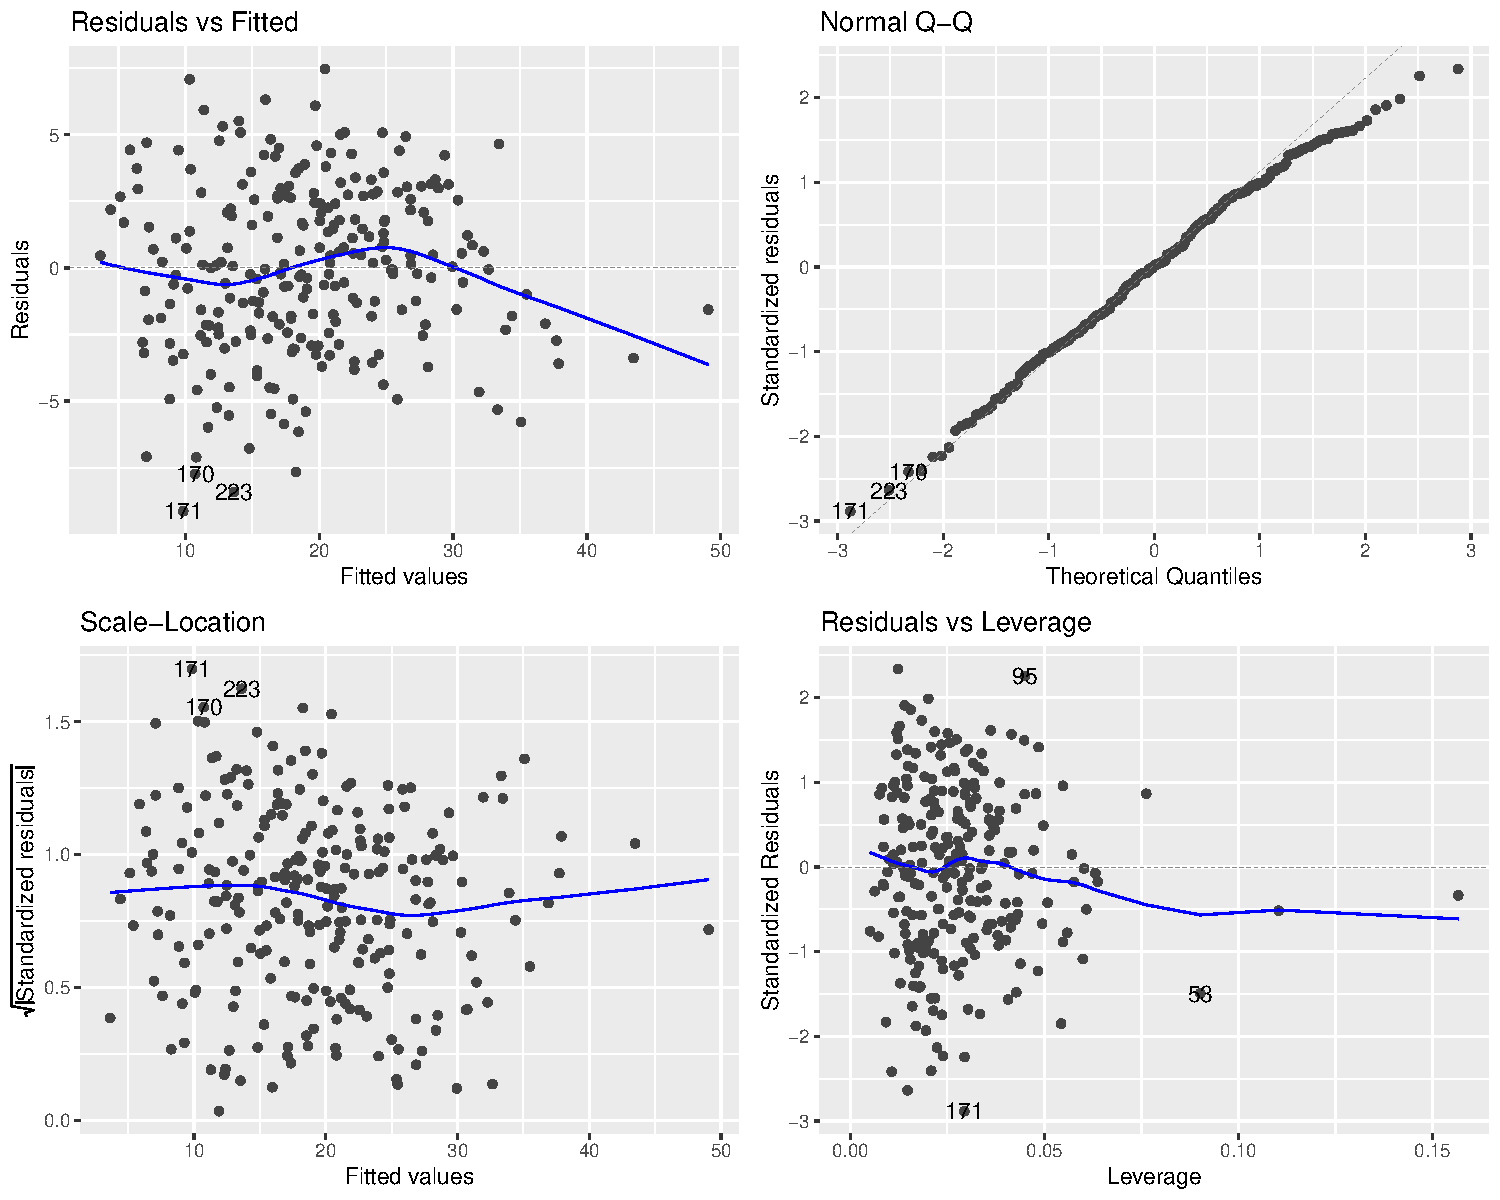
\includegraphics[width=0.95\linewidth]{Images/FIGURES/multivar_linear_regression_final}
	\caption{Multivariate linear regression results diagram for the final model.}
	\label{fig:multivar_linear_regression_final}
\end{figure}


\section{Conclusion}

In this paper an analysis of the population of $252$ men was performed based on their body parts circumference, weight, age and other parameters: 

\begin{itemize}
	\item We have provided descriptive statistics and detailed analysis of selected variables;
	\item Fitting of body fat percentage using multivariate linear regression was carried out.
\end{itemize}

%\newpage{}
%
%\bibliography{bib/Benes2017,bib/MMC}
%
%%\bibliographystyle{plain}
%\bibliographystyle{alpha}

\end{document}
